\chapter{The DREAM Algorithm}
The DREAM algorithm is a Markov Chain Monte Carlo method that is designed for efficient sampling from complex and high-dimensional probability distributions. In this chapter, the algorithm is applied to the hydrological model. The output will then be analyzed and compared to the models from the chapters above.

\section{Algorithm Introduction}
The DREAM algorithm is designed based on the fundamental Metropolis-Hastings algorithm and the possibility of parallel execution of the algorithm. It applies differential evolution. It utilizes multiple Markov chains running in parallel to explore the parameter space. Proposals for new sample points are generated using the differences between pairs of chains. This differential evolution property helps to enhance sampling efficiency and convergence. 


In the first section, we break down the DREAM algorithm step by step with details explained for individual components~\cite{dream}. First, we take a look at the function header. Information regarding input algorithm parameter requirements should be provided.

\begin{algorithm}[H]
function $[x, p\_X]$ \gets \textbf{DREAM}$(prior, pdf, N, n, T, d)$
\end{algorithm}

The DREAM algorithm takes in several parameters as input. These include:
\begin{itemize}
    \item $prior$: The prior distribution of the parameter space.
    \item $pdf$: The probability density function.
    \item $N$: Number of chains.
    \item $n$: Number of generations.
    \item $T$: Thinning factor, which is the implementation of effective sample size in the DREAM algorithm. Only the $T$-th sample will be retained in order to reduce autocorrelation~\cite{dream}.
    \item $d$: Dimension of the inferred parameter space.
\end{itemize}
The output would include $x$, which is the sampled chains positions, and their probabilities, which is denoted by $p_X$.

We move on to the next step, in which variables are initialized.\\

\begin{algorithm}[H]
$[delta, c, c\_star, n\_CR, p\_g] \gets [3, 0.1, 1e-12, 3, 0.2]$\\
$x \gets \textbf{zeros}(T, N, d)$\\
$p\_X \gets \textbf{zeros}(T, N)$\\
$[J, id] \gets [\textbf{zeros}(1, N), 1:N]$\\
\For{$i \gets 1$ \kwTo $N$}{
   $R(:, (i-1) * N + (1:N)) \gets \textbf{setdiff}(1:N, i)$\\
}
$CR \gets [1:n\_CR] / n\_CR$\\
$pCR \gets ones(1, n\_CR) / n\_CR$\\
\end{algorithm}

In this part, most variables that are internally used in this algorithm and not passed as the input algorithm parameters are initialized. These include:
\begin{itemize}
    \item $delta$: Number chain pairs proposal. As mentioned in the introduction of this chapter, this value is used for observing the differential evolution of the sample space.
    \item $p\_g$: The probability of selecting a specific number of pairs of chains for generating the proposals.
    \item $c$: The scaling factor that controls the step size of the proposal distribution.
    \item $c\_star$: The parameter that is used to adaptively update the scaling factor $c$ during sampling, so that an optimal acceptance probability can be controlled.
    \item $J$: The jump rate. It measures the average distance between successive samples in the parameter space and thus quantifies the effectiveness of the parameter space exploration.
    \item $id$: Chain indices that correspond the jump rate.
    \item $CR$: The crossover rate. It is used to determine the proportion of dimensions in which the state of the generated sample differs from the current state.
    \item $n\_CR$: The number of different crossover values. It allows for adaptive updating of the crossover rates during sampling.
    \item $pCR$: The probability of each crossover rate being selected.
\end{itemize}

Next up, we initialize the sample states and probabilities.\\
\begin{algorithm}[H]
$X \gets \textbf{prior}(X, d)$\\
\For{$i \gets 1$ \kwTo $N$}{
    $p\_X(i, 1) \gets pdf(X(i, :))$
}
$x(1, :, 1:d) = \textbf{reshape}(X', [1, N, d]); p\_X(1, 1:N) = p\_X'$
\end{algorithm}

In this segment, the initial states are generated from the prior distribution and stored in $X$. The initial probability of each chain is also computed using the $pdf$ function and stored in $p\_X$. They are then reshaped correspondingly.

From now on, the algorithm enters the sample generation phase. It repeats itself until the completion of sample generation. All of the segments below are wrapped inside of a for loop that repeats until $n$ cycles, which is the number of generation steps. The first segment inside of the loop looks like this:

\begin{algorithm}[H]
$ draw \gets \textbf{sort}(\textbf{rand}(N-1, N))$\\
$dX = \textbf{zeros}(N, d)$\\
$lambda = \textbf{unifrnd}(-c, c, N, 1)$
$std\_X = std(X)$
\end{algorithm}

The $\textbf{unifrnd}$ function is a function that generates random numbers from a uniform distribution. Here, we instantiated another few internal variables.
\begin{itemize}
    \item $draw$: A list of random numbers. They are used to determine the order of chain updates.
    \item $dX$: An array to store proposal differences.
    \item $lambda$: A random variable sampled from a uniform distribution between \(-c\) and \(c\), used for adaptive scaling of the proposal step size.
    \item $std\_X$: The standard deviation of $X$. It is used later for adaptive scaling.
\end{itemize}

Moving on to the next segment, we generate the proposals.

\begin{algorithm}[H]
\For{$i \gets 1 \kwTo N$}{
    $D \gets \textbf{randsample}([1:delta], 1)$\\
    $a = R(i, draw(D, 1))$\\
    $b = R(i, draw(D+1:2*D, 1))$\\
    $d = \textbf{randsample}(1:n\_CR, 1, pCR)$\\
    $z = \textbf{rand}(1, d)$
    $A = find(z <= CR(d))$
    \If{$len(A) == 0$}{
        $A \gets min(z, c\_star = 1)$
    }
    $gamma\_d = 2.38 / sqrt(2 * len(A) * p\_g * (1 - p\_g))$
}
\end{algorithm}

The algorithm loops through every single chain and draws proposals.
\begin{itemize}
    \item $D$: Selects a number of differences for the proposal generation.
    \item $a$, $b$: Chain indices. They are used in the differential evolution proposal.
    \item $d$: Selects a crossover rate using probabilities $pCR$.
    \item $A$: Determines the dimensions that are involved in the crossover. If the dimension turns out to be $0$, we enforce $1$ to be the minimum dimension size.
    \item $gamma\_d$: The scaling factor for the differential evolution proposal. The calculation is based on the number of dimensions and a probability factor $p\_g$.
\end{itemize}

For the next step, the algorithm focuses on the differential evolution proposal. This is one of the most crucial steps of the DREAM algorithm, making it different from other Markov chain Monte Carlo algorithms.

\begin{algorithm}[H]
$g \gets \textbf{randsample}([gamma\_d, 1], 1, [1-p\_g, p\_g])$\\
$dX(i, A) = c\_star + randn(1, len(A)) + (1 + lambda(i)) * g * sum(X(a, A) - X(b, A))$\\
$Xp(i, 1:d) \gets X(i, 1:d) + dX(i, 1:d)$\\
$p\_Xp(i, 1) \gets pdf(Xp(i, :))$\\
$p\_acc \gets \textbf{min}(1, p\_Xp(i, 1) / p\_X(i, 1))$
\end{algorithm}

In this segment, a few calculations is done to decide whether to accept the proposed move. This is done by generating a uniformly distributed random number and accepting the proposed state if this number is less than or equal to the calculated acceptance probability, namely $p_{acc}$.

\begin{itemize}
    \item $g$: Selects a number from $gamma\_d$ or 1.
    \item $dX$: The actual differential evolution proposal, calculated based on the dimension count of $A$, the variability term $lambda$ that is defined above, and the $g$ selected in the row above.
    \item $Xp$: The newly proposed positions.
    \item $p\_Xp$: Density of the newly proposed positions.
    \item $p\_acc$: The acceptance probability, calculated based on the newly proposed positions and their corresponding probabilities using the Metropolis criterion as the fundamental Metropolis-Hastings algorithm.
\end{itemize}

Afterward, we accept or reject the samples that are generated, the same as any other Markov chain Monte Carlo algorithm.

\begin{algorithm}[H]
\If{$rand < p\_acc$}{
    $x(i, 1, :) \gets Xp(i, :)$
    $p\_X(i, 1) \gets p\_Xp(i, 1)$
}
\Else{
    $dX(i, 1:d) \gets 0$
}
$J(i) \gets J(i) sum((dX(i, 1:d) ./ std\_X).^2)$
$id(i) \gets id(i) + 1$
\end{algorithm}

The process of this step is relatively straightforward. A random number is drawn, so that the algorithm can decide if the proposal is accepted. If the proposal is accepted, the position and density of the chain are updated. Otherwise, $dX$ is reset to zero for that chain. Afterwards, the jump rate $J$ and chain index $id$ are updated.

Before ending the repetition and continuing with the next step, there is an extra step in the DREAM algorithm which involves chaining and mixing.

\begin{algorithm}[H]
$x(:, :, :) \gets \textbf{reshape}(X(:, 1:d), [], N, d)$\\
$p\_X(:, 1:N) \gets p\_X.\textbf{transpose}$\\\
\If {$t < T /10$}{
    $pCR \gets 1./J$
    $pCR \gets pCR / \textbf{sum}(pCR)$
}
$[x, p\_X] = \textbf{check}(X, \textbf{mean}(\textbf{log}(p\_X(\textbf{ceil}(T/2):T, :))))$
\end{algorithm}
What the algorithm does in this part is to reshape and update the density of the chain's position for the next iteration. The crossover probabilities $pCR$ are then updated based on the jump rate $J$ to enhance mixing. At the very end, a check function is used to perform outlier detection based on the log probabilities of the chains, removing them and leaving the valuable data inside of the variable.

The loop is then ended. The final step of the algorithm is self-explanatory, namely the return phase. It returns the sampled values in the form of chains and ends itself.
\begin{algorithm}
    $\textbf{return}\  x, p\_X$
\end{algorithm}

The algorithm itself is originally implemented using MATLAB, though it is later rewritten and offered in multiple packages with different implementation variants. For this thesis, the PyDREAM library\footnote{\url{https://pydream.readthedocs.io/en/latest/index.html}} is selected for use. The PyDREAM library brings the DREAM algorithm to the platform of Python with easy installation and usage~\cite{pydream}, which is optimal for the use case of this thesis.

\section{Evaluation Based on Chains}
For the DREAM algorithm, there is a set of default input algorithm parameters. Therefore, before exploring the influence of the input algorithm parameters on the actual output, we first use this set of default input algorithm parameters to run the algorithm to observe how the output of the Bayesian inference looks. Since it is an algorithm based on chains, we analyze the sampled results both with and without regard to chains, analogous to the parallel Metropolis-Hastings algorithm. For the test cases, we test the algorithm using $10$, $8$, $5$, and $4$ chains. Numbers of chains lower than $4$ are not possible due to the policy of the DREAM algorithm, stating that the chain amount must be greater than twice the value of DEpairs + 1. The DEpairs parameter describes the pair of differential evolution and ensures there are enough chains to form the required number of DEpairs for proposal generation.


\subsection{Efficiency}
First, we take a look at the efficiency of the algorithm. We measure the run time for different test cases regarding chain amounts and compare them using graphics, which are displayed below in Figure 8.1. Unlike the parallel Metropolis-Hastings algorithm, there is no strict correlation that can be found between the number of chains and the run time of the DREAM algorithm. The cause is that instead of treating different chains individually, the DREAM algorithm uses cross-over calculations to track the relationships between the different chains. Therefore, the additional calculation results in the irregularity of the efficiency across different test cases of chain amounts.

\begin{figure}[H]
    \centering
    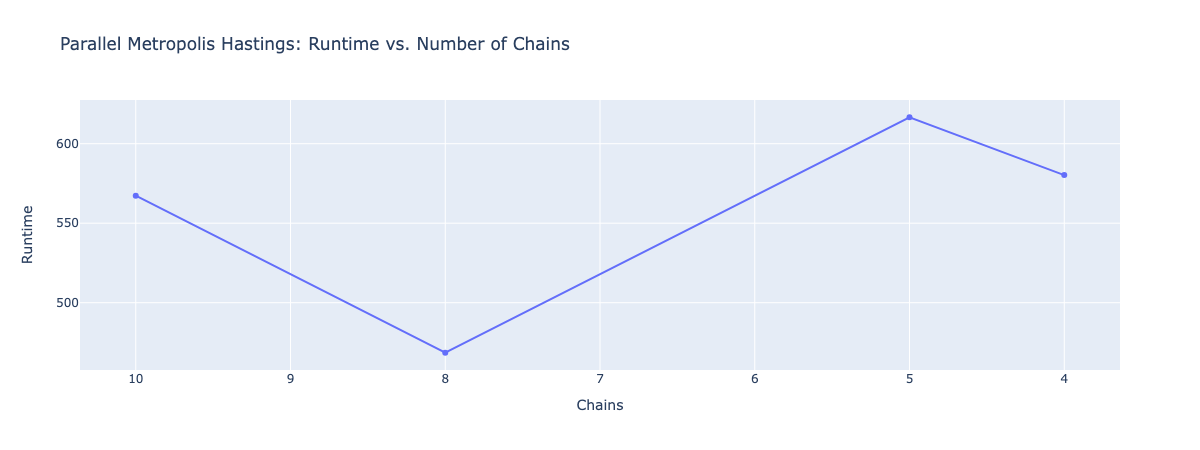
\includegraphics[width=1\textwidth]{figures/dream/runtime.png}
    \captionsetup{width=.8\textwidth}
    \caption{Relationship between run time and chain numbers for the DREAM algorithm}
    \label{fig:enter-label}
\end{figure}
\subsection{Trace Plot}
Similar to the case for the parallel Metropolis-Hastings algorithm evaluation, we use the trace plot to track the positioning of generated samples in each step. For the DREAM algorithm, we also analyze the trace plot of both extreme cases, namely the DREAM algorithm run with $10$ chains and $4$ chains. The trace plots of two random chains picked from both cases are shown in Figures 8.2 to 8.5. Visualizations for both cases do not differ much from each other in terms of sampling from the stationary distribution. All parameters in both graphs show apparent convergence approaching the end, where the stationary distribution can be easily observed. We could conclude that the property of sampling from the stationary distribution of individual chains exists and does not need further investigation.

Unlike the observation made for the parallel Metropolis-Hastings algorithm, the DREAM algorithm displays a heavy stationary distribution, where there are far fewer movements, more rejections during the sampling process, and no obvious moving patterns of the traces. Also, the visualizations show that the parameter space of the stationary distribution from the DREAM algorithm is normally a subset of the entire parameter space, which provides a more stable and consistent sampling, unlike the wide parameter sample space exploration upon stationary distribution in the case of parallel Metropolis-Hastings. In conclusion, the DREAM algorithm has a stronger convergence for the sampling process than other Markov chain Monte Carlo algorithms.

\begin{figure}[H]
    \centering
    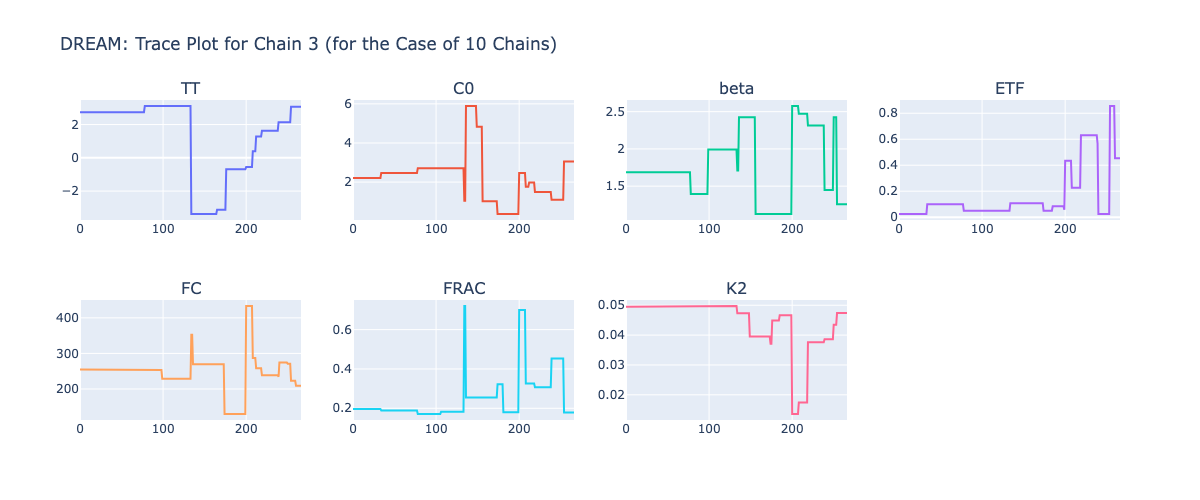
\includegraphics[width=0.8\textwidth]{figures/dream/tp_rand_10_3.png}
    \captionsetup{width=.8\textwidth}
    \caption{Trace plot of the third chain from the DREAM algorithm with 10 chains}
    \label{fig:enter-label}
\end{figure}

\begin{figure}[H]
    \centering
    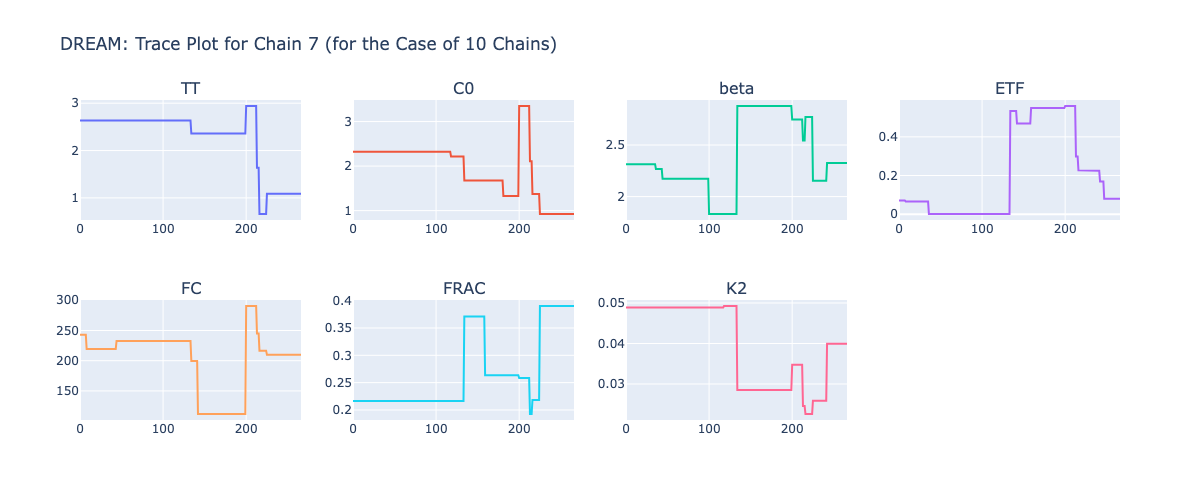
\includegraphics[width=0.8\textwidth]{figures/dream/tp_rand_10_7.png}
    \captionsetup{width=.8\textwidth}
    \caption{Trace plot of the seventh chain from the DREAM algorithm with 10 chains}
    \label{fig:enter-label}
\end{figure}

\begin{figure}[H]
    \centering
    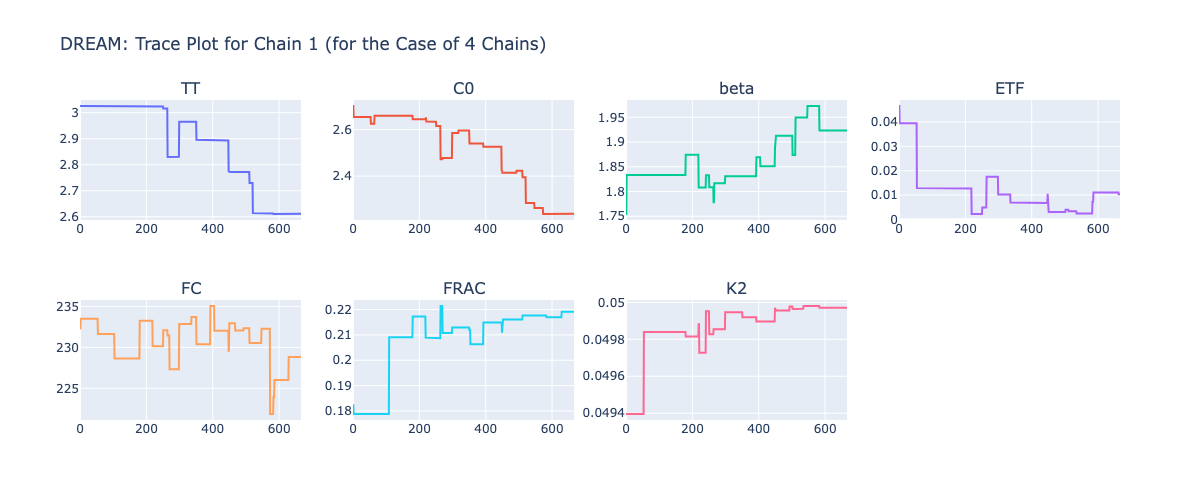
\includegraphics[width=0.8\textwidth]{figures/dream/tp_rand_4_1.png}
    \captionsetup{width=.8\textwidth}
    \caption{Trace plot of the first chain from the DREAM algorithm with 4 chains}
    \label{fig:enter-label}
\end{figure}

\begin{figure}[H]
    \centering
    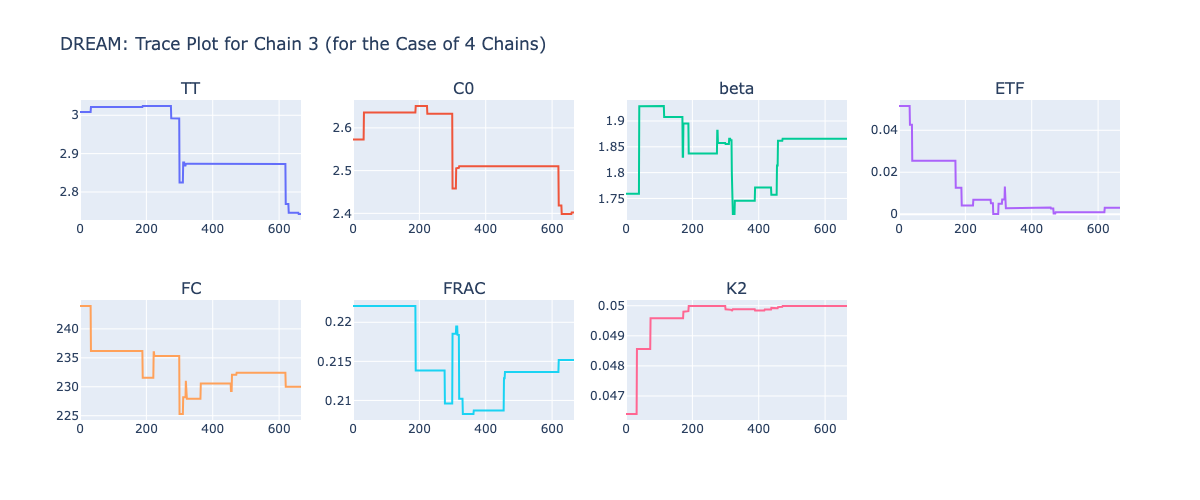
\includegraphics[width=0.8\textwidth]{figures/dream/tp_rand_4_3.png}
    \captionsetup{width=.8\textwidth}
    \caption{Trace plot of the third chain from the DREAM algorithm with 4 chains}
    \label{fig:enter-label}
\end{figure}

\subsection{Gelman Rubin Convergence}
The Gelman Rubin statistic in the case of DREAM is generally higher than the convergence diagnostic of the general parallel Metropolis-Hastings algorithm, even though the convergence statistic is generally in the acceptable range below $1.2$. The figures for all test cases are displayed in Figures 8.6 to 8.9. For the case of 10 chains, two parameters show relatively high convergence diagnostic values that almost exceed the threshold. For other cases, there are also some parameters that show higher convergence diagnostic values than others. However, no specific patterns or regularities can be found for the Gelman-Rubin convergence parameter. 

\begin{figure}[H]
    \centering
    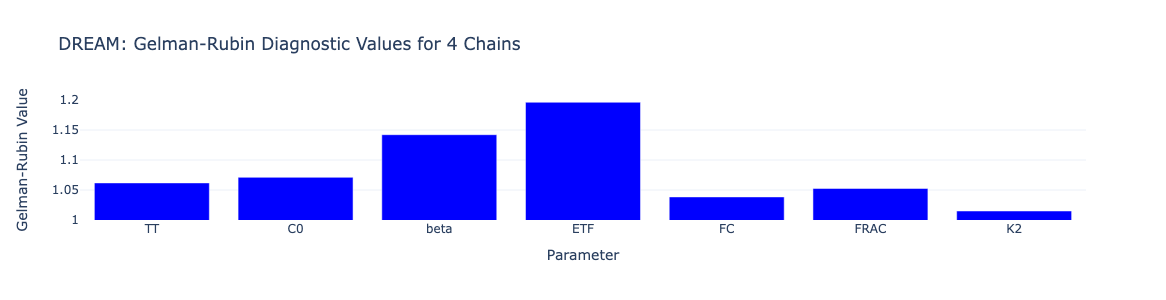
\includegraphics[width=1\textwidth]{figures/dream/gr_10.png}
    \captionsetup{width=.8\textwidth}
    \caption{Gelman Rubin Convergence Diagnostic of the DREAM algorithm with 10 chains}
    \label{fig:enter-label}
\end{figure}

\begin{figure}[H]
    \centering
    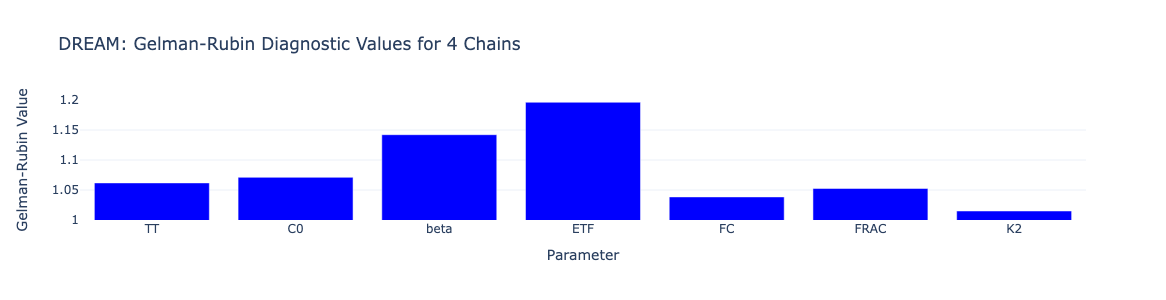
\includegraphics[width=1\textwidth]{figures/dream/gr_8.png}
    \captionsetup{width=.8\textwidth}
    \caption{Gelman Rubin Convergence Diagnostic of the DREAM algorithm with 8 chains}
    \label{fig:enter-label}
\end{figure}

\begin{figure}[H]
    \centering
    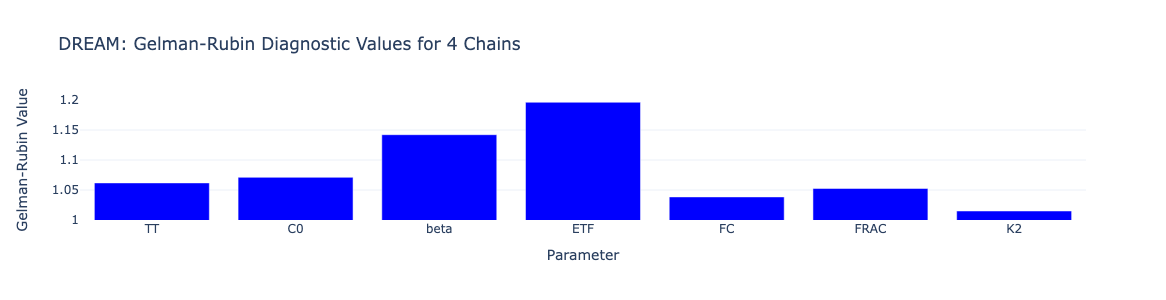
\includegraphics[width=1\textwidth]{figures/dream/gr_5.png}
    \captionsetup{width=.8\textwidth}
    \caption{Gelman Rubin Convergence Diagnostic of the DREAM algorithm with 5 chains}
    \label{fig:enter-label}
\end{figure}

\begin{figure}[H]
    \centering
    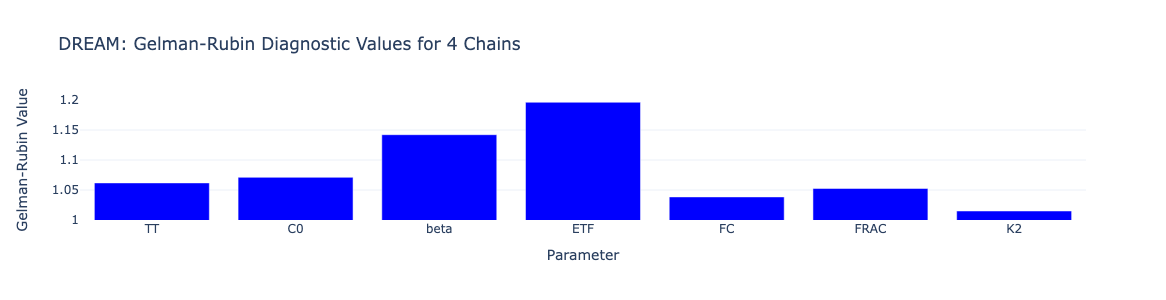
\includegraphics[width=1\textwidth]{figures/dream/gr_4.png}
    \captionsetup{width=.8\textwidth}
    \caption{Gelman Rubin Convergence Diagnostic of the DREAM algorithm with 4 chains}
    \label{fig:enter-label}
\end{figure}

\subsection{Autocorrelation Plot}
We observe the autocorrelation plot for the DREAM algorithm to analyze the degree of sampling independence. At first sight, we can detect drastic different behaviors among all four cases. For the case of $10$ chains in Figure 8.10, the descending of certain parameters is faster than some others. However, the TT and the K2 parameters show a high level of negative correlation, which means that the newly generated samples have potentially an inverse relationship to the samples generated before, indicating the lack of randomness in the sampling process. For the case of $5$ in Figure 8.12 and $4$ chains in Figure 8.13, the final autocorrelation for higher latency is generally in a favorable range. However, most parameters don't display a rapid descending, which might lead to inefficient sampling and longer convergence. The case of $8$ chains displays the best autocorrelation plot among all four, including fast decrement and low level of autocorrelation throughout the entire range of latency.
\begin{figure}[H]
    \centering
    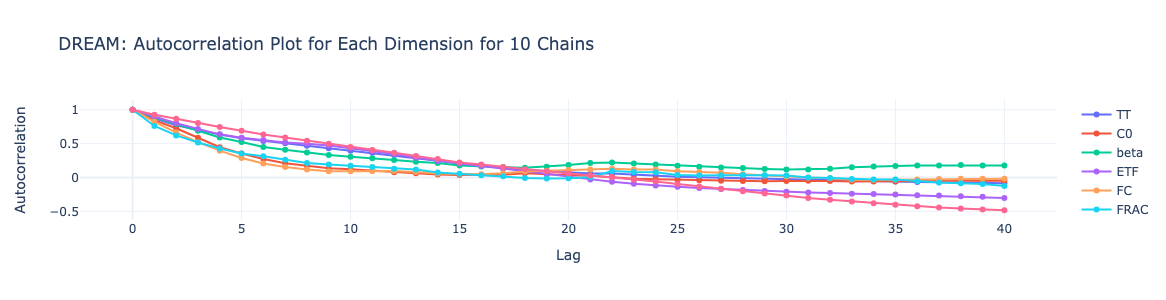
\includegraphics[width=1\textwidth]{figures/dream/ac_10.png}
    \captionsetup{width=.8\textwidth}
    \caption{Autocorrelation plot of the DREAM algorithm with 10 chains}
    \label{fig:enter-label}
\end{figure}

\begin{figure}[H]
    \centering
    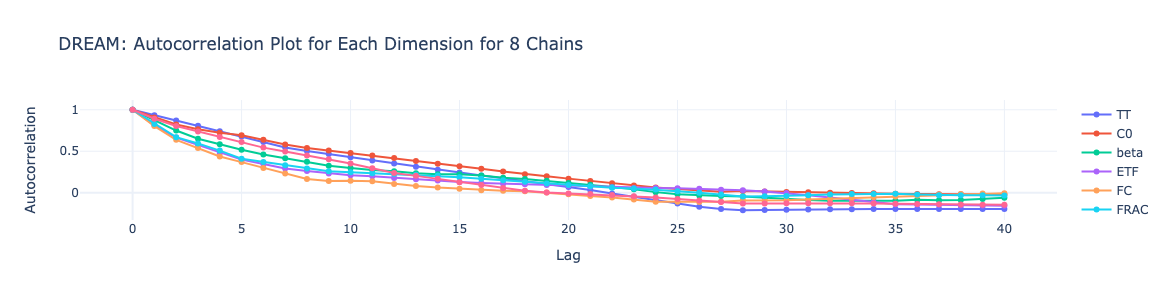
\includegraphics[width=1\textwidth]{figures/dream/ac_8.png}
    \captionsetup{width=.8\textwidth}
    \caption{Autocorrelation plot of the DREAM algorithm with 8 chains}
    \label{fig:enter-label}
\end{figure}

\begin{figure}[H]
    \centering
    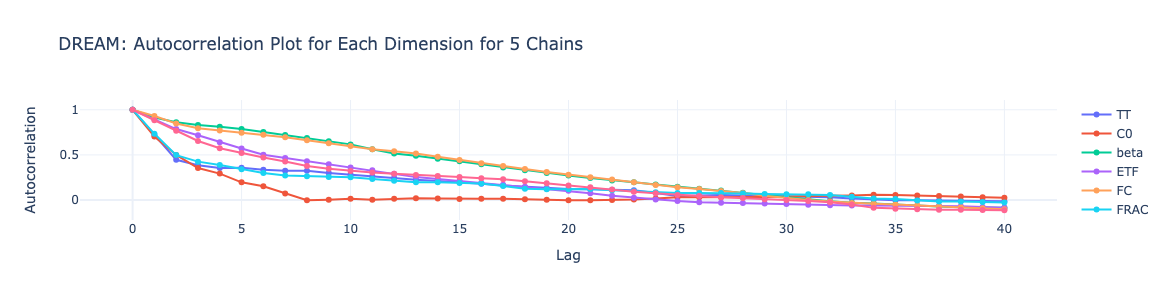
\includegraphics[width=1\textwidth]{figures/dream/ac_5.png}
    \captionsetup{width=.8\textwidth}
    \caption{Autocorrelation plot of the DREAM algorithm with 5 chains}
    \label{fig:enter-label}
\end{figure}

\begin{figure}[H]
    \centering
    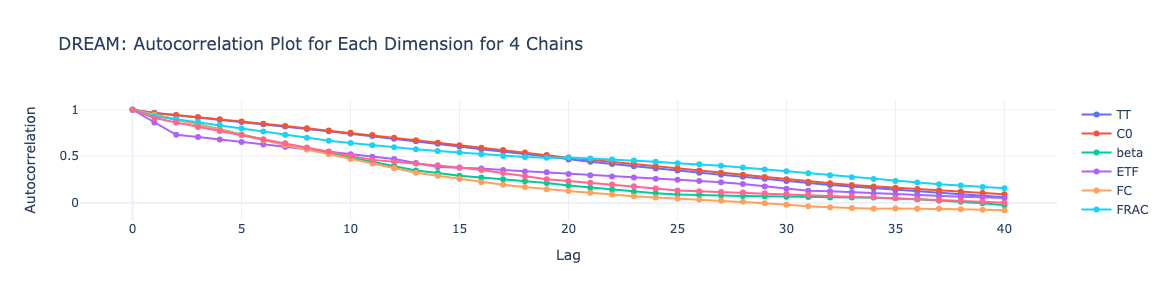
\includegraphics[width=1\textwidth]{figures/dream/ac_4.png}
    \captionsetup{width=.8\textwidth}
    \caption{Autocorrelation plot of the DREAM algorithm with 4 chains}
    \label{fig:enter-label}
\end{figure}


\subsection{Accuracy}
The accuracy metrics including RMSE mean and MAE mean are also gathered for all test cases. The line plot of the RMSE mean displayed in 7.14 shows irregularity of the accuracy of the metric, with the accuracy scores for each test case being very close to each other. For the line plot of the MAE mean displayed in 7.15, a clear ascending pattern can be found. The more chains there are, the more accurate the Bayesian inference will be, though by a small difference.
\begin{figure}[H]
    \centering
    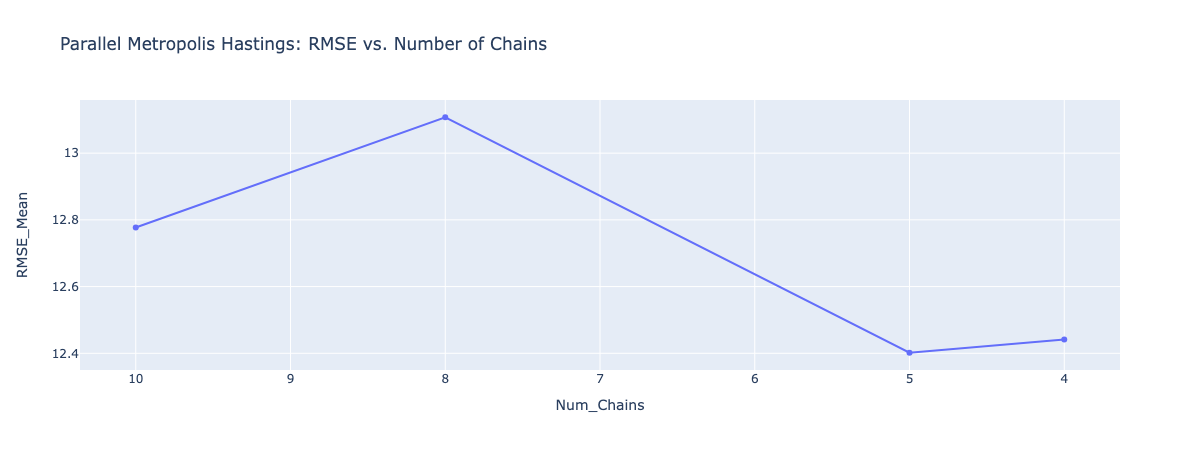
\includegraphics[width=1\textwidth]{figures/dream/rmse.png}
    \captionsetup{width=.8\textwidth}
    \caption{Mean RMSE of the DREAM algorithm across test cases with different chains}
    \label{fig:enter-label}
\end{figure}

\begin{figure}[H]
    \centering
    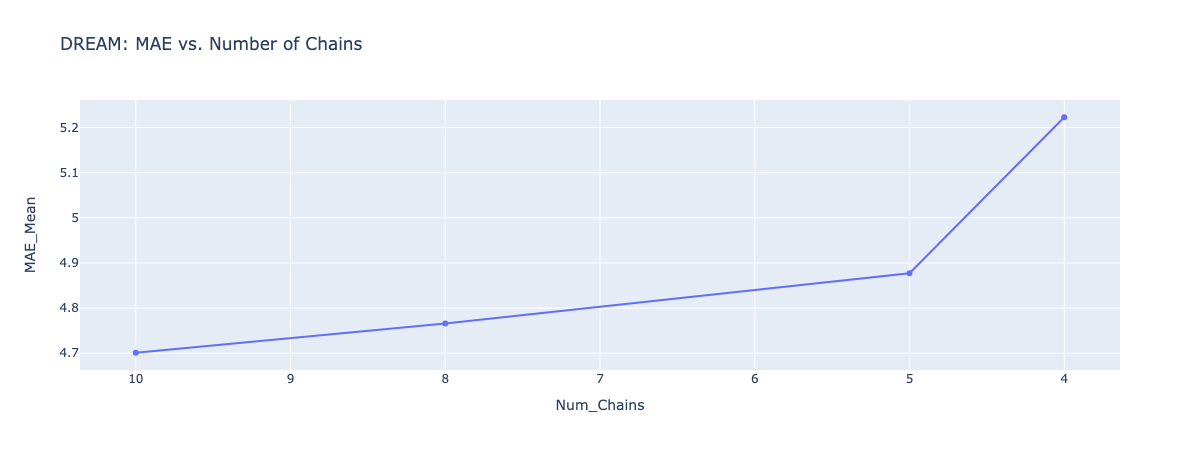
\includegraphics[width=1\textwidth]{figures/dream/mae.png}
    \captionsetup{width=.8\textwidth}
    \caption{Mean MAE of the DREAM algorithm across test cases with different chains}
    \label{fig:enter-label}
\end{figure}

\subsection{Parameter Overview}
Moving on to the last section of the chain analysis, which is the parameter overview. Like the parallel Metropolis-Hastings algorithm, both distribution plots and boxplots are shown here. The focus here is put on the case of $10$ chains and $4$ chains, both extreme cases. 

From the distribution visualization displayed in Figures 8.16 and 8.18, most of the chains for the same parameter have a peak in the region where the most samples are generated in the combined sample collection, with a few exceptions. For instance, for the TT parameter of the case of $10$ chains, all of the chains display a peak near the higher bound for its sample space, which corresponds to the peak at the same position for the combined sample space. This is also the case for the C0 parameter for the test case of $10$ chains, with the peak situated at around the position of 25\% quantile. The exception here is the $7$th chain, which is the only chain among all that does not have a peak there. The above-described scenario is opposite to the case of the parallel Metropolis-Hastings algorithm, in which each chain explores different areas of the parameter space. We can therefore find out the strong correlation between the sampling for each single chain and combined sample space.

For the boxplot displayed in Figures 8.17 and 8.19, however, the visualization shows no pattern at all. For some parameters like ETF from the test case of $4$ chains or K2 from the test case of $10$ chains, the medians across all chains are at around the same position. However, for the majority of cases, absolutely no regularity can be found to show where the positions of the 25\% quantile, the median, and the 50\% quantile are. Therefore, further investigation of the boxplot is not necessary.

\begin{figure}[H]
    \centering
    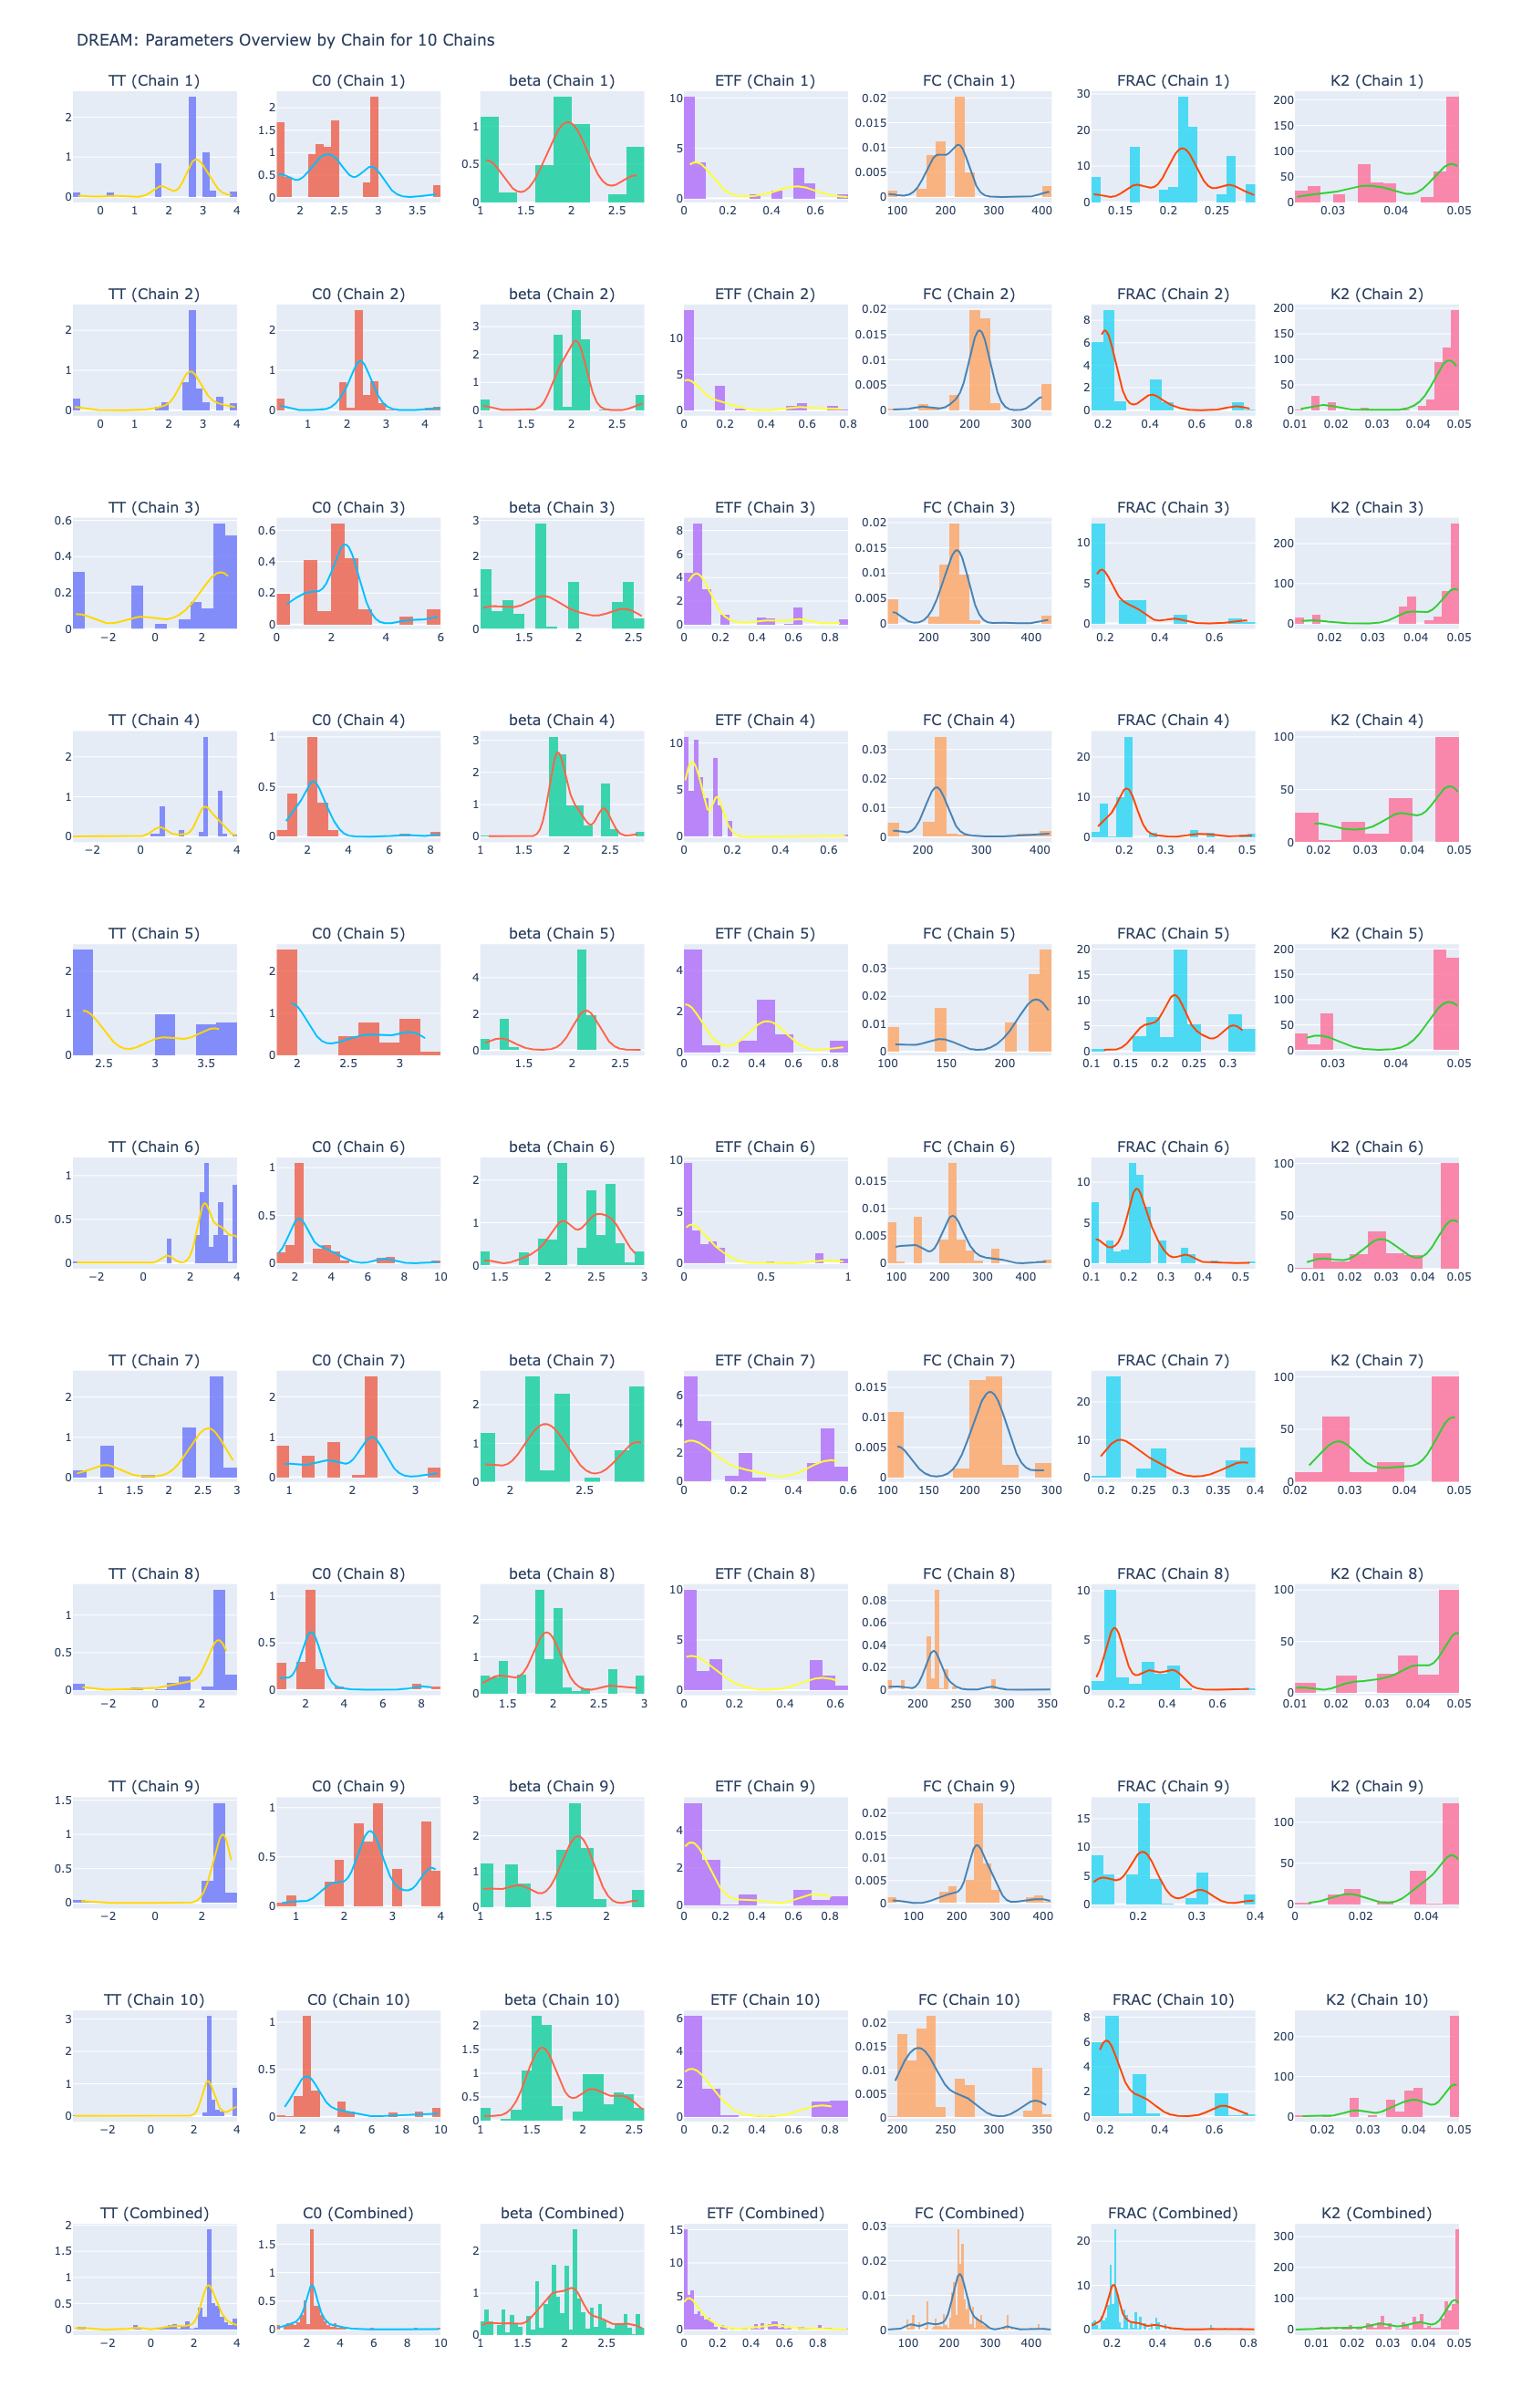
\includegraphics[width=0.8\textwidth]{figures/dream/param_overview_10.png}
    \captionsetup{width=.8\textwidth}
    \caption{Parameter overview by chain for DREAM using 10 chains}
    \label{fig:enter-label}
\end{figure}

\begin{figure}[H]
    \centering
    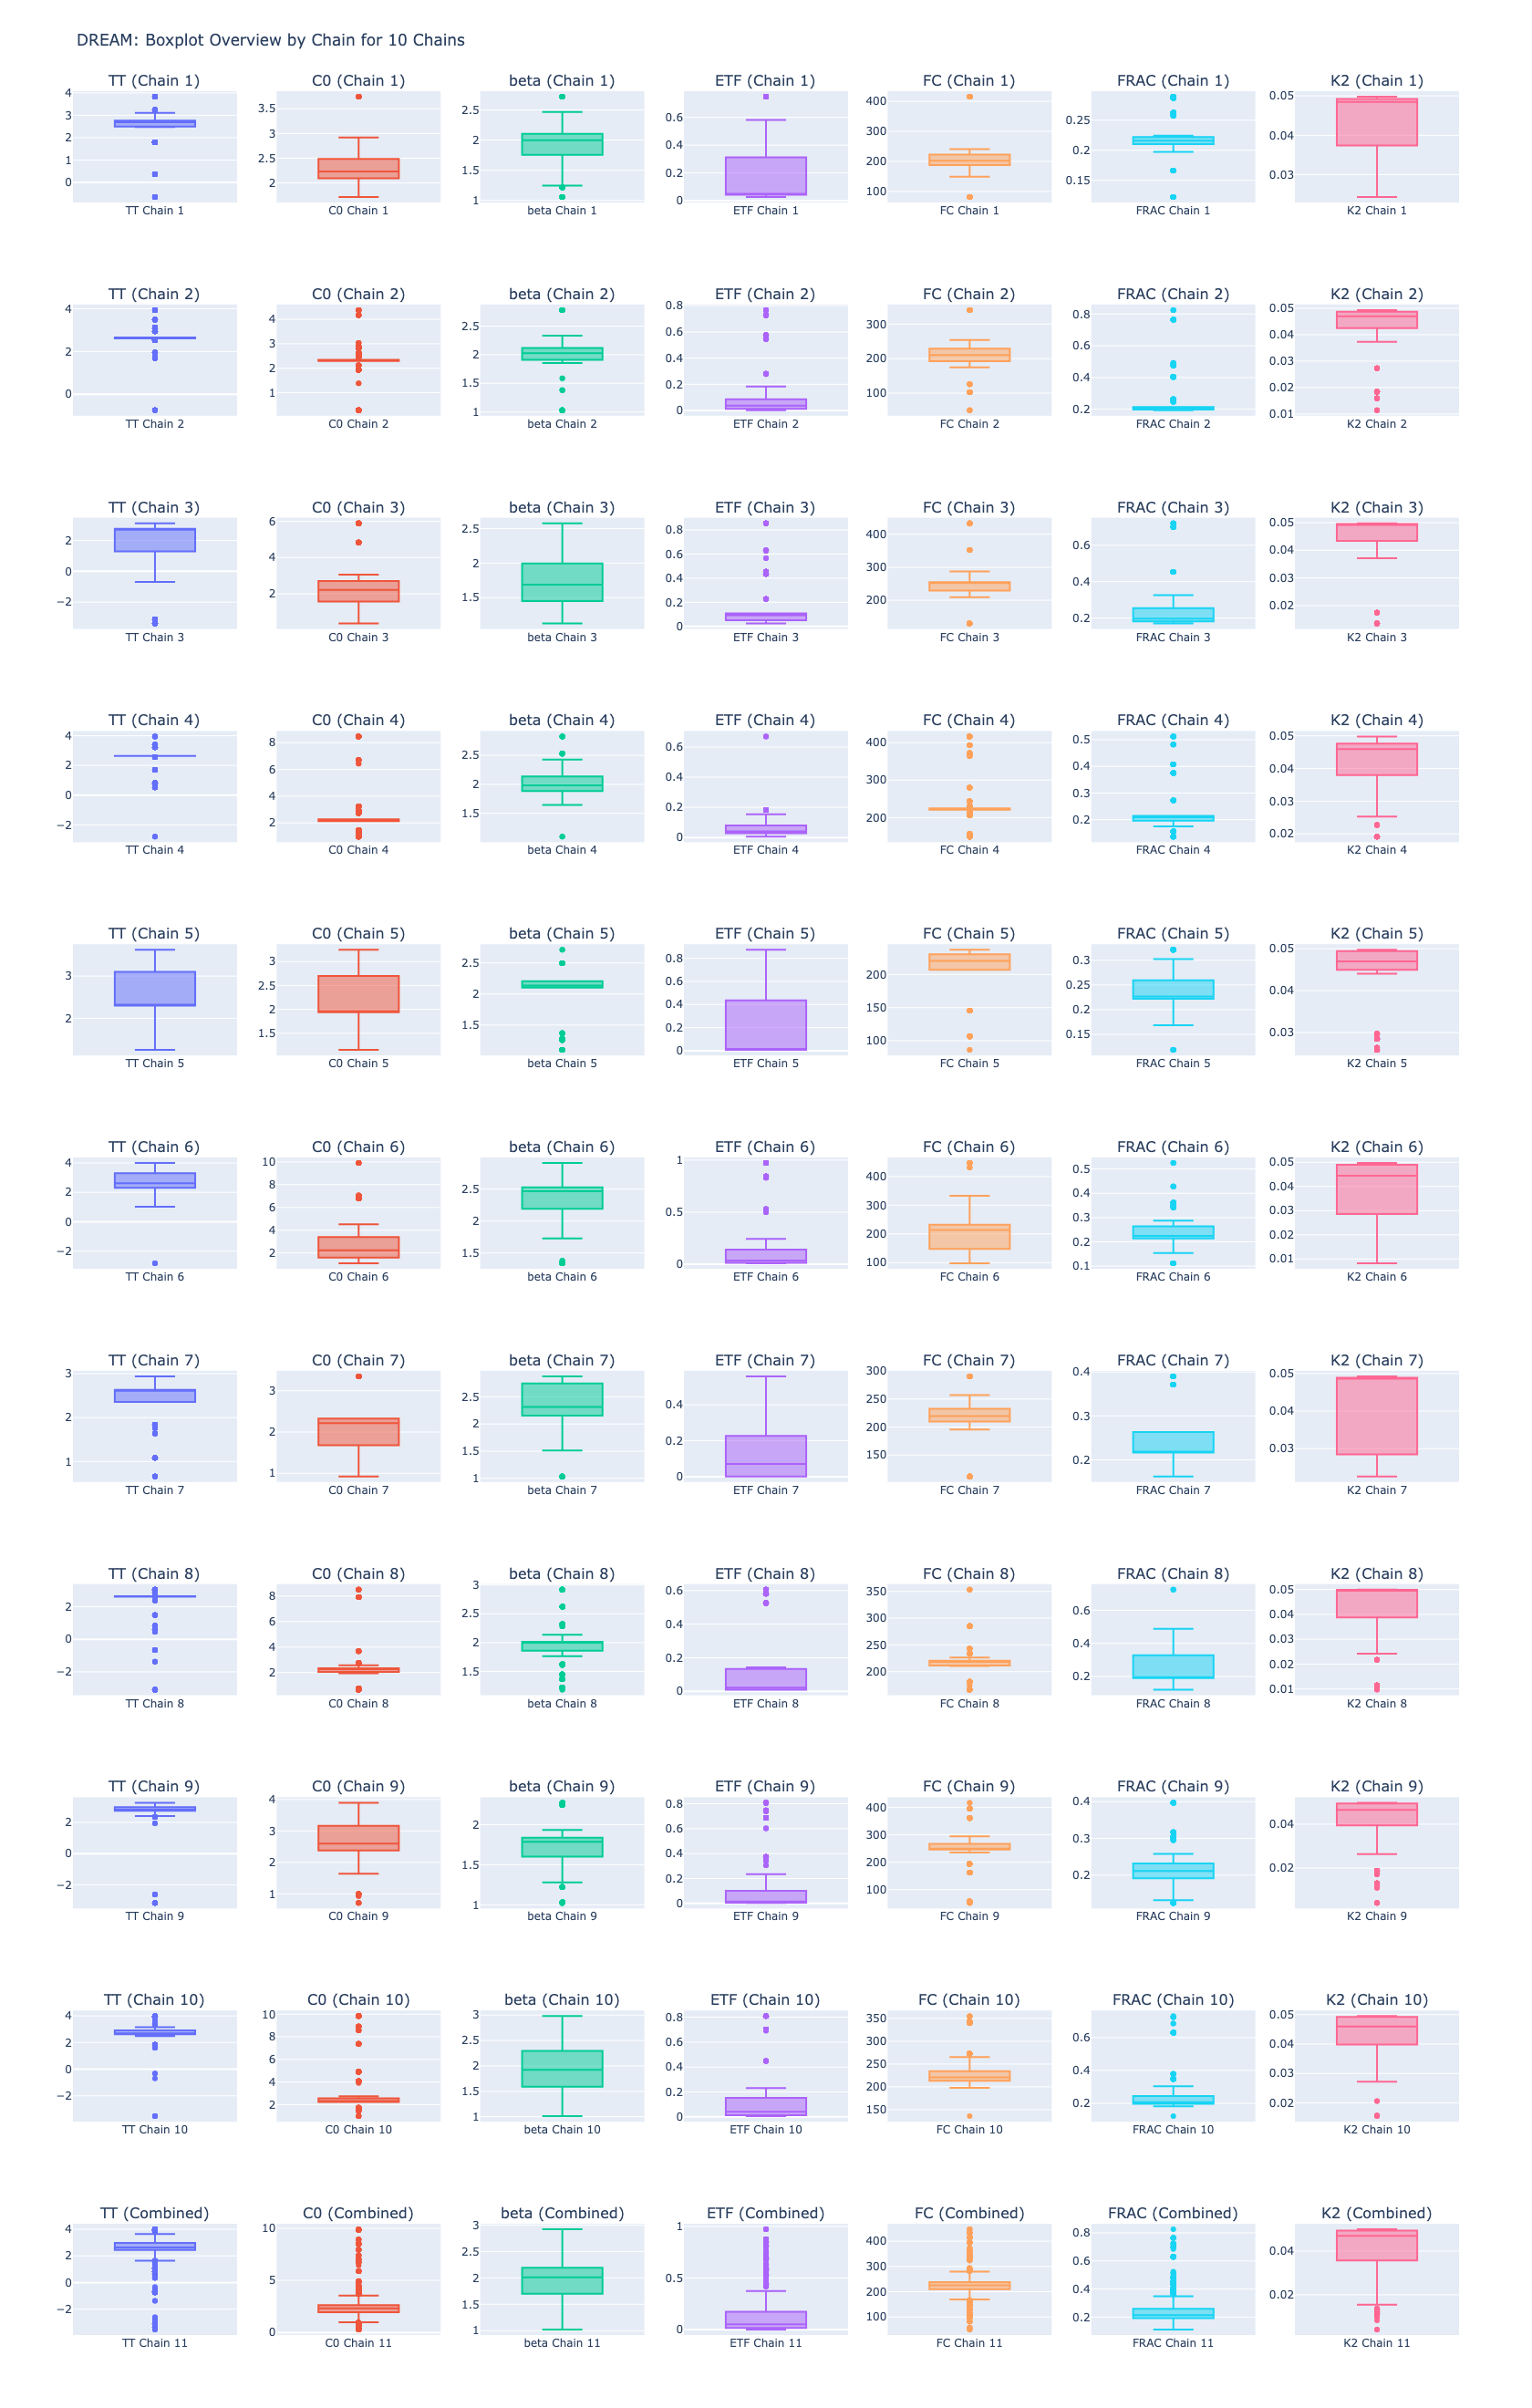
\includegraphics[width=0.8\textwidth]{figures/dream/boxplot_10.png}
    \captionsetup{width=.8\textwidth}
    \caption{Boxplot by chain for DREAM using 10 chains}
    \label{fig:enter-label}
\end{figure}

\begin{figure}[H]
    \centering
    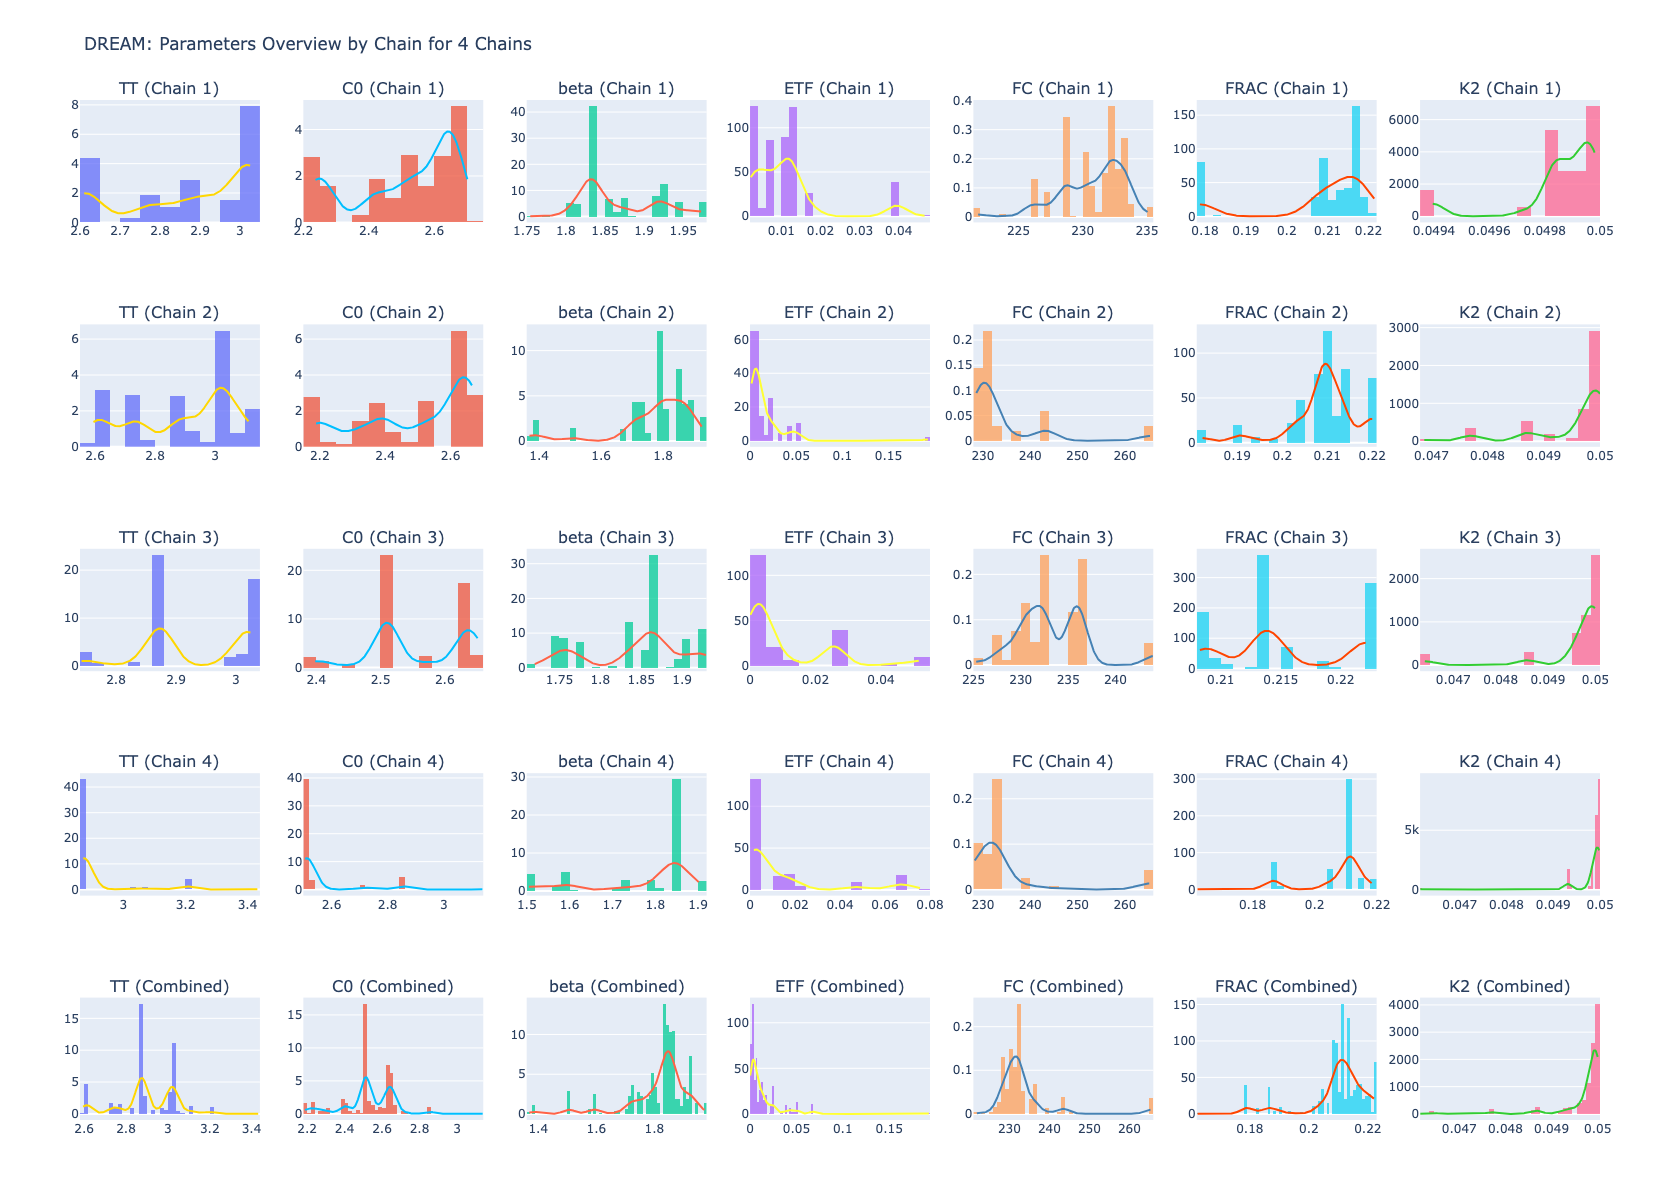
\includegraphics[width=0.6\textwidth]{figures/dream/param_overview_4.png}
    \captionsetup{width=.8\textwidth}
    \caption{Parameter overview by chain for DREAM using 4 chains}
    \label{fig:enter-label}
\end{figure}

\begin{figure}[H]
    \centering
    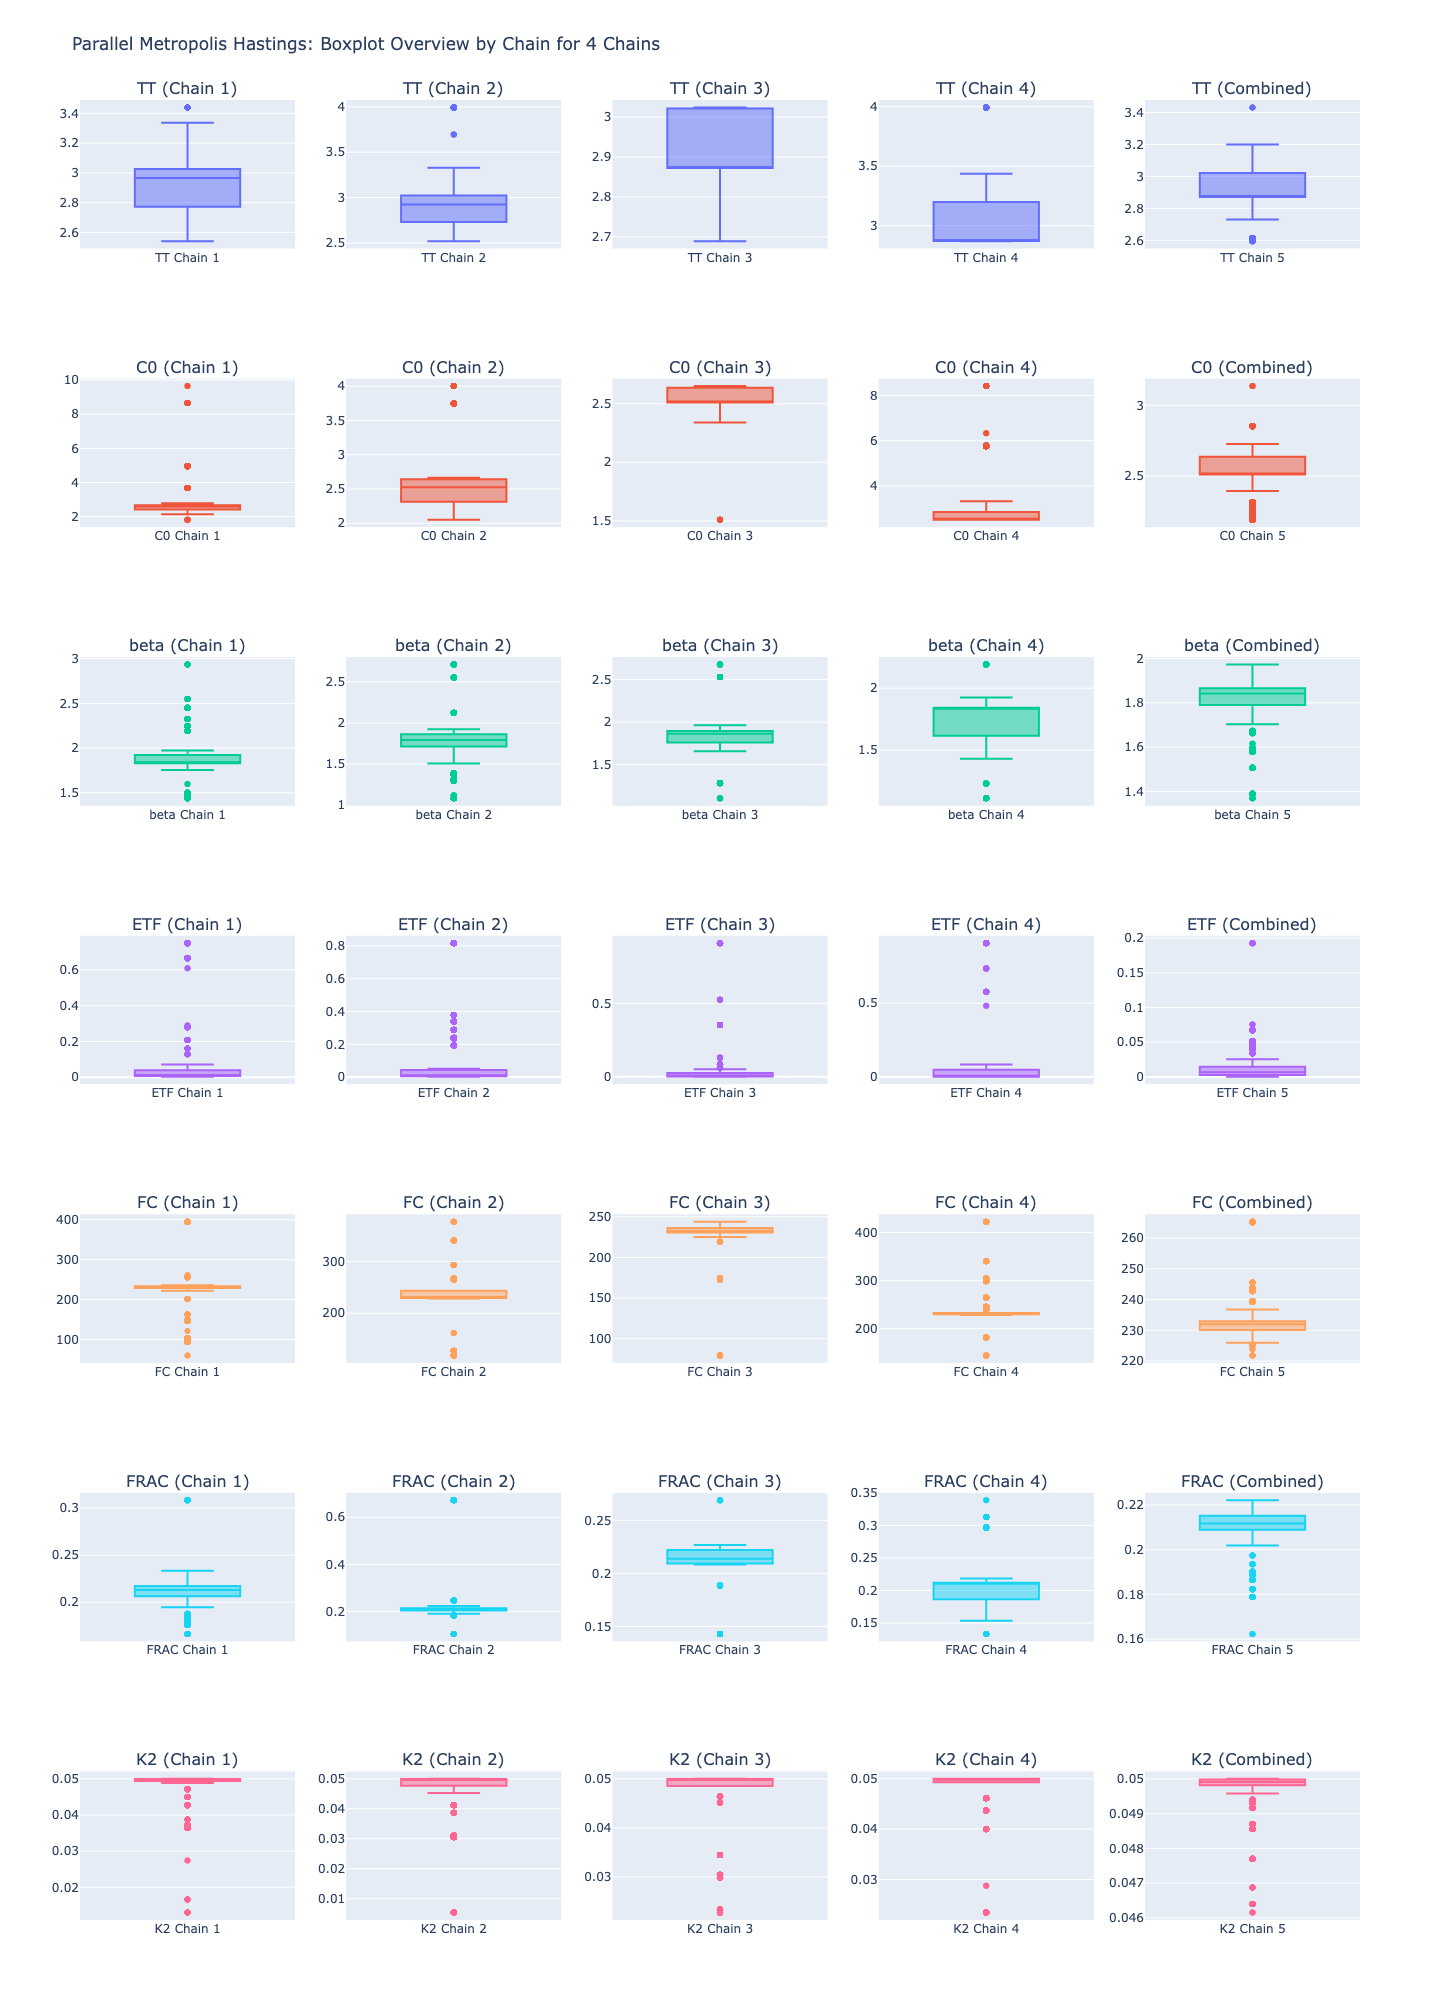
\includegraphics[width=0.6\textwidth]{figures/dream/boxplot_4.png}
    \captionsetup{width=.8\textwidth}
    \caption{Boxplot by chain for DREAM using 4 chains}
    \label{fig:enter-label}
\end{figure}

\section{Input Algorithm Parameters Exploration}
The last part of this chapter is the input algorithm parameter exploration for the DREAM algorithm. Being different from the other Markov chain Monte Carlo algorithms, the DREAM algorithm has a few input algorithm parameters that are unique to itself, with another few that are identical to the ones that the other Markov chain Monte Carlo algorithms possess. Explanation alongside analysis of benchmark data are listed below in smaller sections. 

\subsection{Sampling out of Bounds}
The first input algorithm parameter that is investigated is the handling of the sampling out of bounds, which also exists for all of the other algorithms mentioned in this thesis. For the DREAM algorithm, this parameter is called HardBoundaries, which determines whether the samples that are generated out of bounds are going to be reflected or ignored. The result is listed in Figure 8.20, where both results show relatively close accuracy and efficiency scores to each other. Even though not by much, the method of reflection performs generally better than the method of ignoring, which makes it a better choice for most use cases of the DREAM algorithm.

\begin{figure}[H]
    \centering
    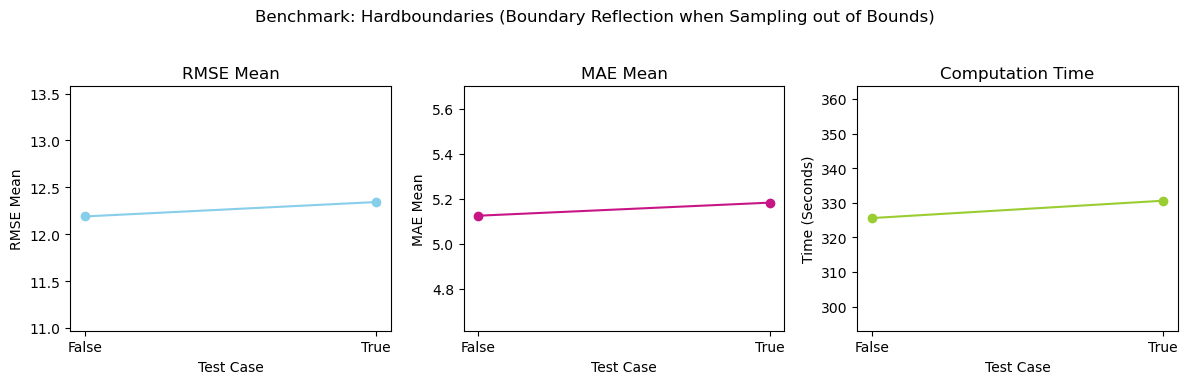
\includegraphics[width=1\textwidth]{figures/dream/sotb.png}
    \captionsetup{width=.8\textwidth}
    \caption{Comparison of the accuracy and the efficiency of DREAM algorithms based on the HardBoundaries parameter}
    \label{fig:enter-label}
\end{figure}

\subsection{Crossover}

In the DREAM algorithm, the concept of crossover is adapted from evolutionary algorithms and specifically implemented to enhance the proposal mechanism in comparison to other Markov chain Metropolis-Hastings algorithms. It is a process of combining information from multiple chains to create new proposal candidates, during which the components of the proposal vector are selectively swapped with corresponding components from other chains based on a crossover probability~\cite{dream}. This method helps the algorithm explore the parameter space more efficiently by utilizing differences between chains.

The crossover burn-in is one of the aspects of the crossover concept. It denotes the number of iterations to fit the crossover values, ensuring the algorithm sufficiently adjusts and optimizes the crossover probabilities for effective parameter space exploration. The default value of this input algorithm parameter in PyDREAM is 10\%. For testing purposes, however, the algorithm is also run with 0\% (which is denoted as NaN in PyDREAM), 20\%, and 50\%. From the figure shown in 7.21, however, not much differences between the metric scores of all of the configurations are shown, apart from the slightly worse efficiency score of the 0\% case against all of the other cases. This input algorithm parameter has, therefore, not that much influence on the Bayesian inference result.
\begin{figure}[H]
    \centering
    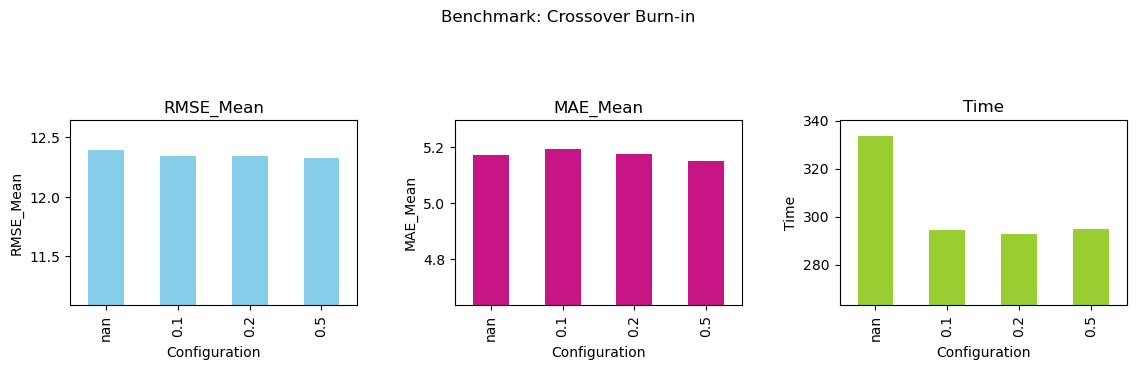
\includegraphics[width=1\textwidth]{figures/dream/crossover_burn_in.png}
    \captionsetup{width=.8\textwidth}
    \caption{Comparison of the accuracy and the efficiency of DREAM algorithms based on the crossover burn in parameter}
    \label{fig:enter-label}
\end{figure}

Another aspect would be the adaptive crossover, which is responsible for the decision to adjust the crossover probabilities based on the performance of the chains~\cite{dream}. This adaptation helps maintain an optimal balance between exploration and exploitation of the parameter space. By default, this option is set, even though we can also turn it off. The algorithm is therefore run in both variants, with the benchmark visualization displayed in Figure 8.22. However, there is only minimal difference between the metric scores of both variants, which is completely neglectable. 
\begin{figure}[H]
    \centering
    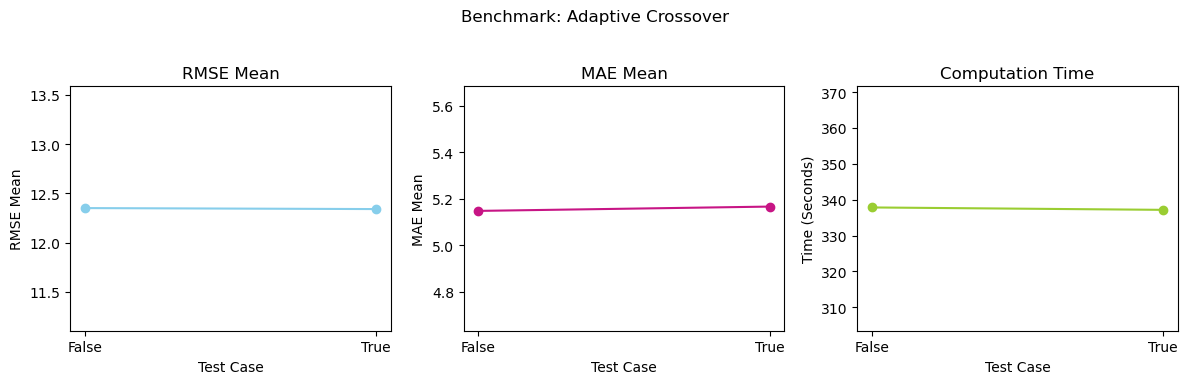
\includegraphics[width=1\textwidth]{figures/dream/adaptive_crossover.png}
    \captionsetup{width=.8\textwidth}
    \caption{Comparison of the accuracy and the efficiency of DREAM algorithms based on the adaptive crossover parameter}
    \label{fig:enter-label}
\end{figure}

For the last aspect of the cross-over, we observe the nCR input algorithm parameter, which defines the number of crossover values to sample from during the run and to fit during the crossover burn-in period. Its default value is set as $3$ for PyDREAM, whereas we also test two other cases, namely $1$ and $3$. From Figure 8.23, the differences between all these three cases are also neglectable, just as adaptive crossover. However, the default value of $3$ generally provides worse metric scores, both in terms of accuracy and efficiency.
\begin{figure}[H]
    \centering
    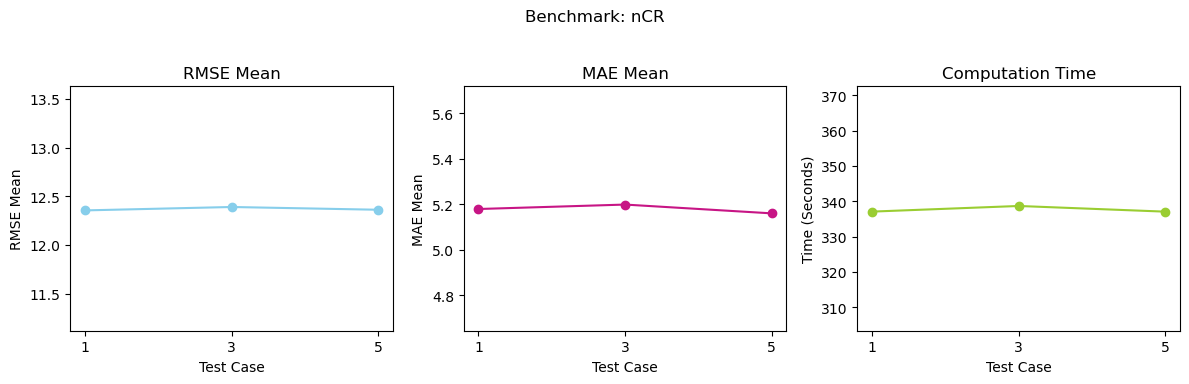
\includegraphics[width=1\textwidth]{figures/dream/nCR.png}
    \captionsetup{width=.8\textwidth}
    \caption{Comparison of the accuracy and the efficiency of DREAM algorithms based on the nCR parameter}
    \label{fig:enter-label}
\end{figure}

\subsection{Likelihood Kernel}
The likelihood kernel function is manually defined for the DREAM algorithm, just as any other Markov chain Monte Carlo algorithm. An investigation here is therefore also necessary. We keep the likelihood kernel in the same format as the one used in other algorithms, with two available options that include independent and dependent versions.

For the dependent version, the best accuracy performance happens at low likelihood kernel factors, with the metric inaccuracy growing as the factor grows, even though the differences are also neglectable. However, the computation time of the factor $5$ is the most optimal, being almost 20 seconds faster than other test cases. This efficiency difference could play an important role in the selection of value.

For the independent version, the best accuracy performance happens at $0.6$. There are, however, no patterns that can be found. For the computation time, the efficiency grows as the factor value grows. However, the independent version of the likelihood function performs much worse than the dependent version of the likelihood function, both in RMSE and in MAE metrics. Therefore, this version of the likelihood function is not considered in the case of the DREAM algorithm.
\begin{figure}[H]
    \centering
    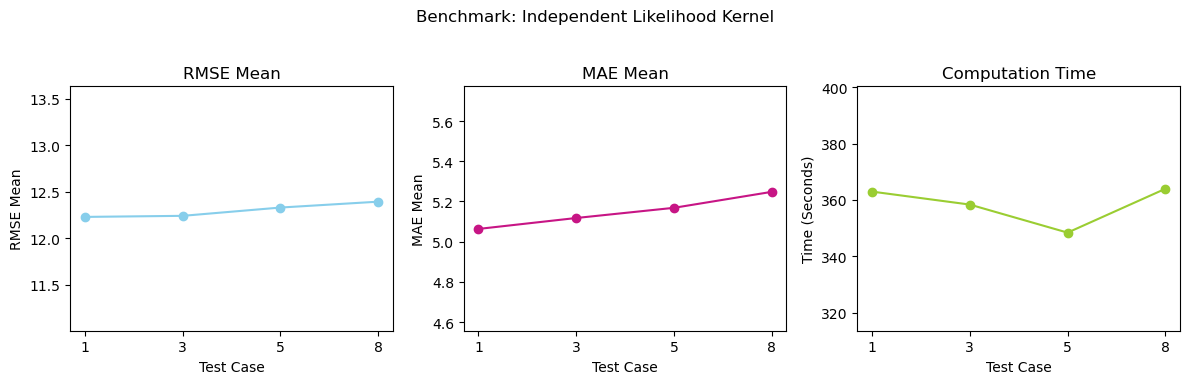
\includegraphics[width=1\textwidth]{figures/dream/indp_likelihood.png}
    \captionsetup{width=.8\textwidth}
    \caption{Comparison of the accuracy and the efficiency of DREAM algorithms based on the independent likelihood kernel factor}
    \label{fig:enter-label}
\end{figure}

\begin{figure}[H]
    \centering
    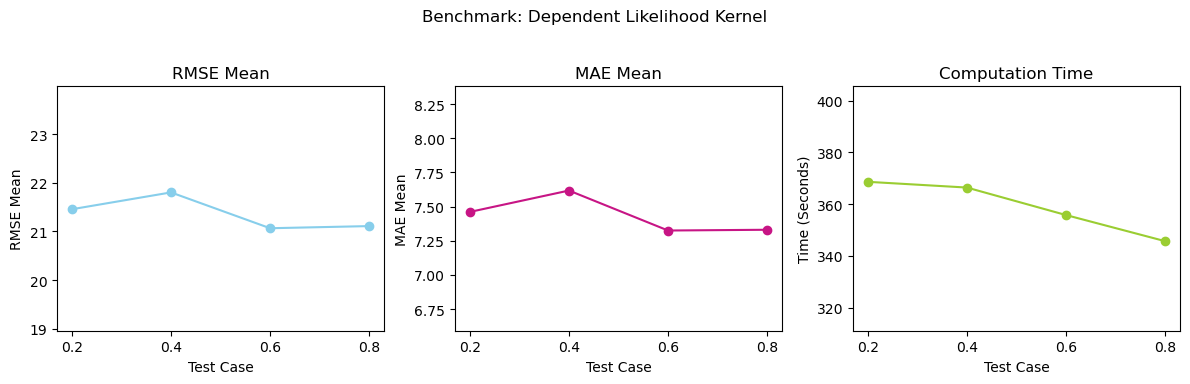
\includegraphics[width=1\textwidth]{figures/dream/dp_likelihood.png}
    \captionsetup{width=.8\textwidth}
    \caption{Comparison of the accuracy and the efficiency of DREAM algorithms based on the dependent likelihood kernel factor}
    \label{fig:enter-label}
\end{figure}

\subsection{Initialization}
The initialization method is a big topic for efficiency enhancement. It is no exception for the case of the DREAM algorithm. The same initialization methods as other algorithms are proposed and used here. The visualization is then displayed in Figure 8.26. As expected, the accuracy metrics do not differ much from each other. However, the most efficient initialization methods according to the efficiency metrics are lower bound, upper bound, $1$st quantile of the prior distribution, the mean of the prior distribution, $3$rd quantile of the prior distribution, and the $1$st quantile of the posterior distribution.
\begin{figure}[H]
    \centering
    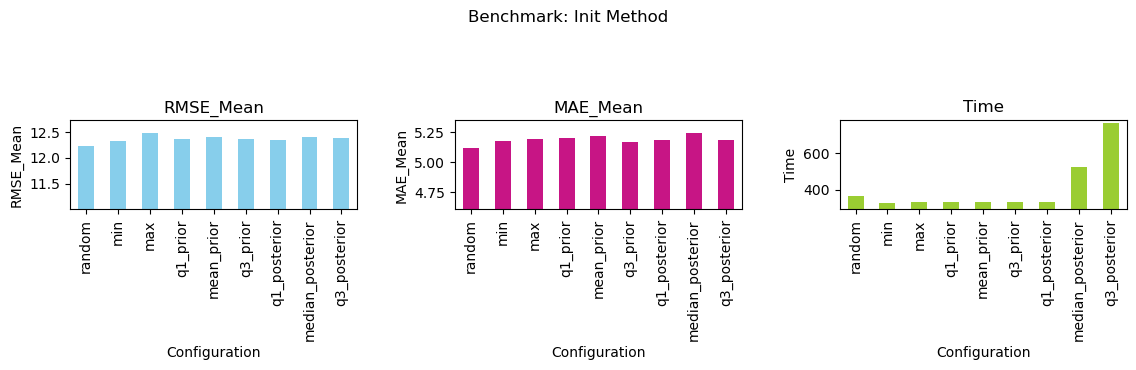
\includegraphics[width=1\textwidth]{figures/dream/init.png}
    \captionsetup{width=.8\textwidth}
    \caption{Comparison of the accuracy and the efficiency of DREAM algorithms based on the initialization method}
    \label{fig:enter-label}
\end{figure}


\subsection{Gamma}
In the DREAM  algorithm, the parameter gamma controls the step size in the proposal generation process, which determines how far the new proposals can move from the last sample. When gamma equals 1, the updates are larger, which enables the algorithm to make broader moves, allowing the algorithm to avoid local extreme points and improve the chain mixing. In PyDREAM, the parameter to adjust is called p\_gamma\_unity, which specifies the probability that gamma will be set to 1 during the sample generation. By adjusting it, we can balance between exploration with larger steps and exploration with smaller steps, making the sampling process able to be customized for specific use cases and requirements. The default probability of p\_gamma\_level is 20\%, whereas all values between $0$ and $1$ with a distance of $0.2$ are used for testing purposes. Figure 8.27 documents the benchmarked data in a visual way, from which we can directly infer that the default value of $0.2$ and the other value of $0.8$ deliver good RMSE scores, where $0.8$ outperforms the $0.2$ case by MAE, though not by much. For the run time, however, there is indeed a noticeable difference, where the configuration of $0$, $0.2$, and $1$ all deliver a more ideal efficiency score than other test cases.

\begin{figure}[H]
    \centering
    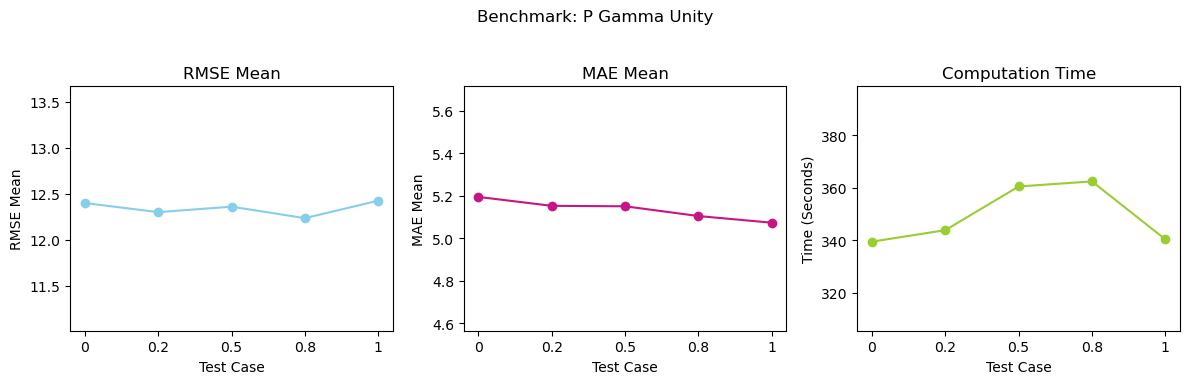
\includegraphics[width=1\textwidth]{figures/dream/gamma.png}
    \captionsetup{width=.8\textwidth}
    \caption{Comparison of the accuracy and the efficiency of DREAM algorithms based on the p gamma unity parameter}
    \label{fig:enter-label}
\end{figure}

\subsection{Differential Evolution}
Differential Evolution (DE) is an optimization algorithm that iteratively enhances a population of candidate solutions by generating new candidates through the weighted difference between pairs of existing solutions (DEpairs) and combining them with a third solution. In the DREAM algorithm, DEpairs ensure diverse and effective exploration of the parameter space, while the snooker update further enhances exploration by projecting vector differences onto the current state, helping to navigate complex, multimodal distributions. Together, these mechanisms enable robust and efficient optimization in high-dimensional problems.

In the DREAM algorithm, differential evolution is an optimization method that improves the sampling candidate solutions by generating new samples using the weighted difference between pairs of existing samples and then using the crossover to mix components of these solutions. Using this method, provides robustness for the algorithm, ensuring it can explore complex and high-dimensional parameter spaces efficiently. To tune the DREAM algorithm with respect to differential evolution, there are two input algorithm parameters available. These are discussed in the following subsections.

\subsubsection{DEpairs}
In the introduction part, the concept of using the weighted difference between pairs of existing samples is mentioned. The amount of sample pairs is called DEpairs, which is responsible for generating new samples that keep maintain the diversity in the sample result and the good mixing of the chains. By default, only one pair of existing samples is chosen for the calculation. For testing purposes, other values including $2$ and $3$ are tested, so that we can observe to which extent the number of pairs affects the Bayesian inference result. The benchmark data is recorded as visualization in Figure 8.28, where we can infer that using $2$ pairs of existing samples provides slightly better accuracy both in terms of RMSE and MAE than the rest of the pair amounts. The computation time is, however, a complete reflection of the accuracy metrics, where using $1$ or $3$ pairs of existing samples provides an overall better efficiency than the case of $2$. Thus, the selection of value here is a trade-off between accuracy and efficiency.

\begin{figure}[H]
    \centering
    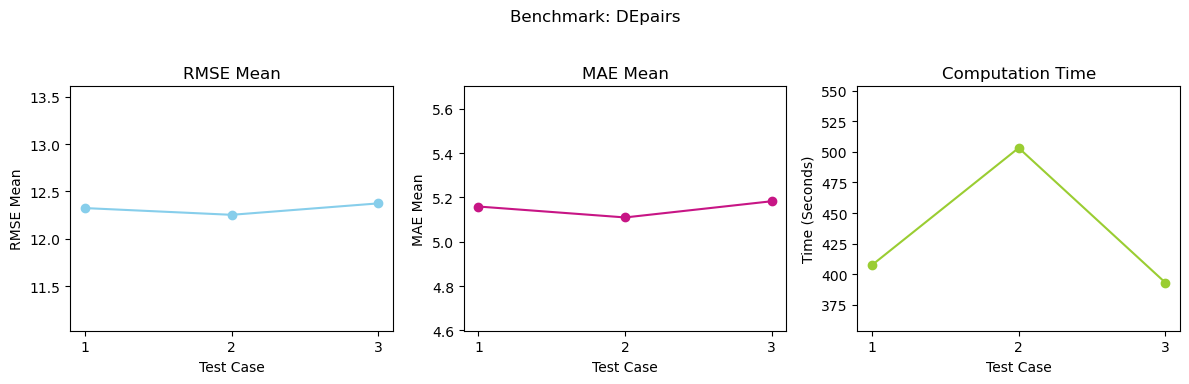
\includegraphics[width=1\textwidth]{figures/dream/DEpairs.png}
    \captionsetup{width=.8\textwidth}
    \caption{Comparison of the accuracy and the efficiency of DREAM algorithms based on the DEpairs parameter}
    \label{fig:enter-label}
\end{figure}

\subsubsection{Snooker}
Another mechanism in terms of differential evolution that is applied in the DREAM algorithm, other than the above-mentioned pairs inference, is the snooker update. It further enhances exploration by projecting vector differences between two chains onto the current state instead of randomly selecting pairs for further sampling. In the DREAM algorithm, a probability is set for the algorithm to determine whether to use a snooker update instead of a regular update for the next iteration, since a snooker update is more compute-heavy. The default probability is set as 10\%, whereas we test different values including 20\%, 50\%, and 80\%. Besides, the two extreme cases are also tested, where we completely ditch the idea of snooker update and only keep the regular updates based on randomly selecting pairs (0\%), and where we only use snooker update in each iteration (100\%). The benchmark data is stored in Figure 8.29. For efficiency, there is not much difference between the run time across all configurations. For the accuracy metric, on the other hand, the extreme case of not using the snooker update delivers the best performance in comparison with other cases, where the snooker update is partially or completely used. The conclusion is then drawn, that for the use case of the hydrological model, not using the snooker update delivers a more accurate result.
\begin{figure}[H]
    \centering
    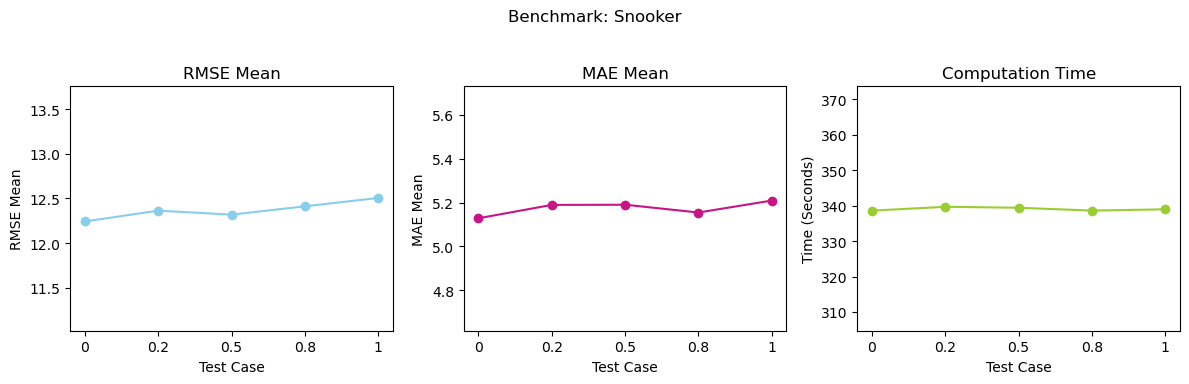
\includegraphics[width=1\textwidth]{figures/dream/snooker.png}
    \captionsetup{width=.8\textwidth}
    \caption{Comparison of the accuracy and the efficiency of DREAM algorithms based on the snooker parameter}
    \label{fig:enter-label}
\end{figure}

\subsection{Burn In Phase}
Burn-in phase is another crucial topic for all Markov chain Monte Carlo algorithms. From the analysis in the chapters above, the burn-in phase poses a great influence on the outcome of the Bayesian inference, therefore it is also investigated here. The benchmark result is visualized in Figure 8.30. For the aspect of accuracy, we pick the factor over 5, which is the 20\% burn-in phase. The relationship between the efficiency metrics and the configuration is, on the other hand, the complete opposite of the relationship between accuracy metrics and the configuration. The lower factor, which is the 50\% burn-in phase, results in a more efficient run time than the higher factor, which is the 20\% burn-in phase. The selection of the burn-in phase amount then also becomes a trade-off between accuracy and efficiency.
\begin{figure}[H]
    \centering
    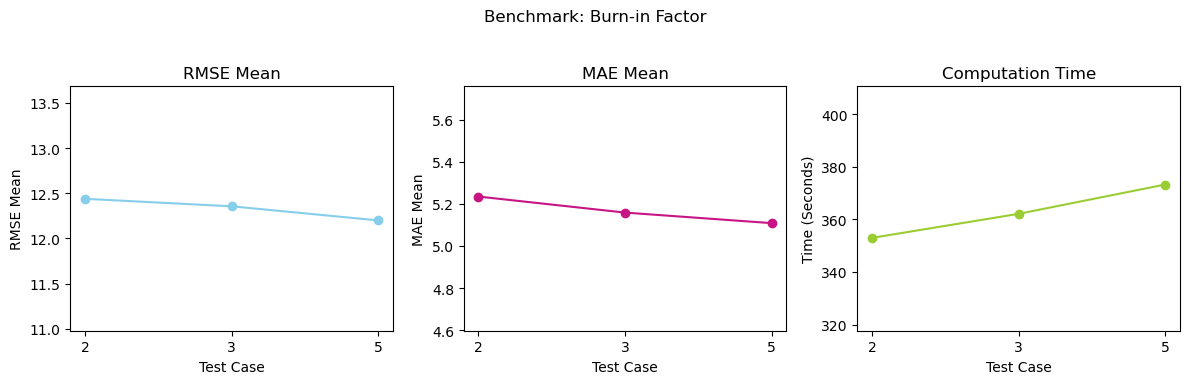
\includegraphics[width=1\textwidth]{figures/dream/burn_in.png}
    \captionsetup{width=.8\textwidth}
    \caption{Comparison of the accuracy and the efficiency of DREAM algorithms based on the burn in factor}
    \label{fig:enter-label}
\end{figure}

\subsection{Effective Sample Size}
Unlike the burn-in input algorithm parameter, the effective sample size shows no patterns that can be found. From the graph shown in Figure 8.31, the only information that is presented is the most optimal configuration for accuracy score, namely the effective sample size of $5$, and also the best configuration in terms of efficiency, namely the effective sample size of $2$, $4$ and $5$.
\begin{figure}[H]
    \centering
    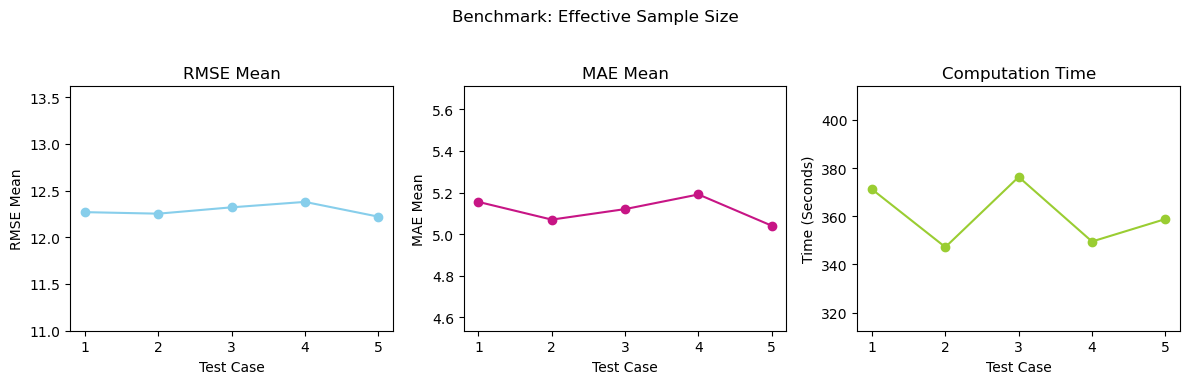
\includegraphics[width=1\textwidth]{figures/dream/ess.png}
    \captionsetup{width=.8\textwidth}
    \caption{Comparison of the accuracy and the efficiency of DREAM algorithms based on the effective sample size}
    \label{fig:enter-label}
\end{figure}

\section{Result and Comparison with Other Algorithms}
Same as the case for the general parallel Metropolis-Hastings algorithm, the dream algorithm is also run one more time, so that we can gather the data output for visualization. A comparison with the other algorithms is going to be made, both in terms of accuracy and efficiency.

The overview of the posterior distribution after the calibration is shown in the first graph, where the generated samples are more concentrated than in the posterior generated by the general parallel Metropolis-Hastings algorithm. This suggests that the DREAM algorithm has a higher efficiency in exploring the parameter space, leading to more precise estimations of the posterior distributions. The increased concentration of samples suggests a more reliable convergence and leads to better efficiency of the calibration process. Altogether with the concentration of the aggregation of generated samples from each dimension, the DREAM algorithm is the best choice in terms of the parameter calibration under uncertainty, exceeding the general parallel Metropolis-Hastings algorithm.

\begin{figure}[H]
    \centering
    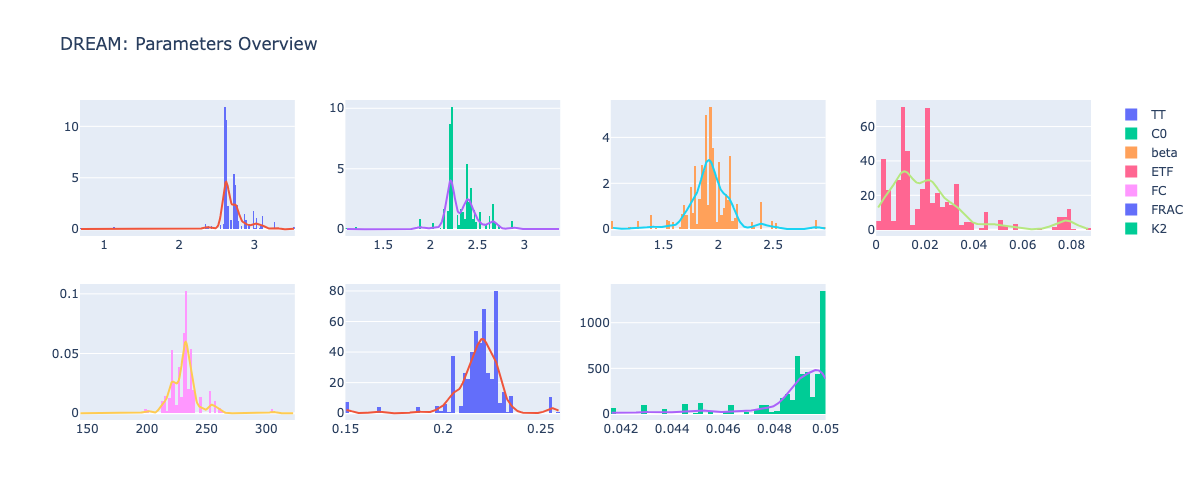
\includegraphics[width=1\textwidth]{figures/dream/paramter_overview.png}
    \captionsetup{width=.8\textwidth}
    \caption{Overview of the posterior distribution of the parameters calibrated by the general parallel Metropolis-Hastings algorithm}
    \label{fig:enter-label}
\end{figure}

\begin{figure}[H]
    \centering
    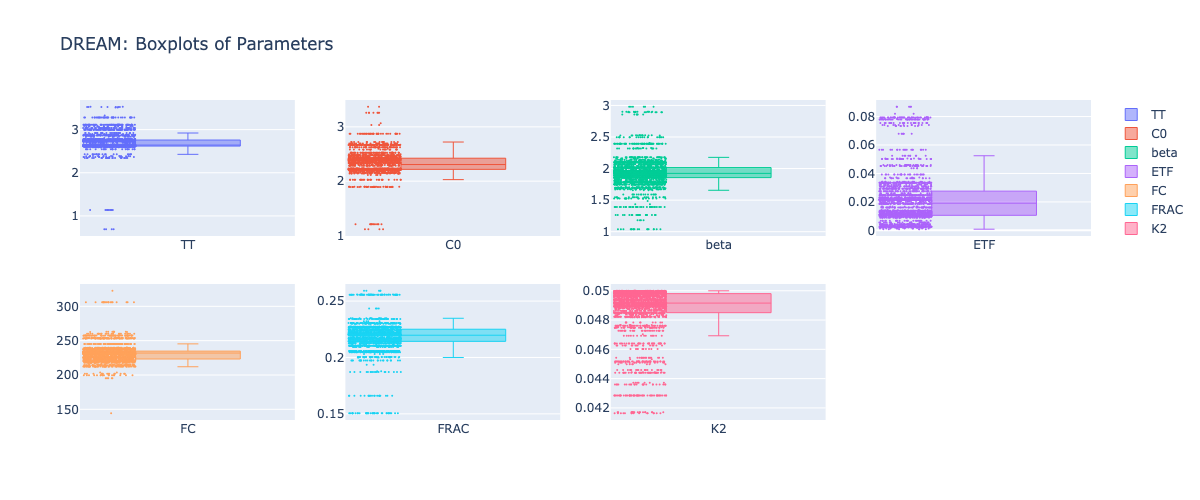
\includegraphics[width=1\textwidth]{figures/dream/boxplot.png}
    \captionsetup{width=.8\textwidth}
    \caption{Boxplots of the generated posterior samples of each parameter calibrated by the general parallel Metropolis-Hastings algorithm}
    \label{fig:enter-label}
\end{figure}

In terms of accuracy, the RMSE score of the algorithm is around $20$ and the MAE score is around $9$ for most cases, which is a slight downgrade from the general parallel Metropolis-Hastings algorithm. Considering the extreme boost regarding the efficiency, with an average runtime of around $400$ seconds against $4000$ seconds, the DREAM algorithm would be an optimal choice for the uncertainty quantification.